% Options for packages loaded elsewhere
\PassOptionsToPackage{unicode}{hyperref}
\PassOptionsToPackage{hyphens}{url}
%
\documentclass[
  10pt,
]{scrbook}
\usepackage{amsmath,amssymb}
\usepackage{lmodern}
\usepackage{iftex}
\ifPDFTeX
  \usepackage[T1]{fontenc}
  \usepackage[utf8]{inputenc}
  \usepackage{textcomp} % provide euro and other symbols
\else % if luatex or xetex
  \usepackage{unicode-math}
  \defaultfontfeatures{Scale=MatchLowercase}
  \defaultfontfeatures[\rmfamily]{Ligatures=TeX,Scale=1}
  \setmonofont[Scale=0.8]{Source Code Pro}
\fi
% Use upquote if available, for straight quotes in verbatim environments
\IfFileExists{upquote.sty}{\usepackage{upquote}}{}
\IfFileExists{microtype.sty}{% use microtype if available
  \usepackage[]{microtype}
  \UseMicrotypeSet[protrusion]{basicmath} % disable protrusion for tt fonts
}{}
\makeatletter
\@ifundefined{KOMAClassName}{% if non-KOMA class
  \IfFileExists{parskip.sty}{%
    \usepackage{parskip}
  }{% else
    \setlength{\parindent}{0pt}
    \setlength{\parskip}{6pt plus 2pt minus 1pt}}
}{% if KOMA class
  \KOMAoptions{parskip=half}}
\makeatother
\usepackage{xcolor}
\IfFileExists{xurl.sty}{\usepackage{xurl}}{} % add URL line breaks if available
\IfFileExists{bookmark.sty}{\usepackage{bookmark}}{\usepackage{hyperref}}
\hypersetup{
  pdftitle={LaTeX Dersleri},
  pdfauthor={Zafer Acar},
  hidelinks,
  pdfcreator={LaTeX via pandoc}}
\urlstyle{same} % disable monospaced font for URLs
\usepackage{color}
\usepackage{fancyvrb}
\newcommand{\VerbBar}{|}
\newcommand{\VERB}{\Verb[commandchars=\\\{\}]}
\DefineVerbatimEnvironment{Highlighting}{Verbatim}{commandchars=\\\{\}}
% Add ',fontsize=\small' for more characters per line
\usepackage{framed}
\definecolor{shadecolor}{RGB}{248,248,248}
\newenvironment{Shaded}{\begin{snugshade}}{\end{snugshade}}
\newcommand{\AlertTok}[1]{\textcolor[rgb]{0.94,0.16,0.16}{#1}}
\newcommand{\AnnotationTok}[1]{\textcolor[rgb]{0.56,0.35,0.01}{\textbf{\textit{#1}}}}
\newcommand{\AttributeTok}[1]{\textcolor[rgb]{0.77,0.63,0.00}{#1}}
\newcommand{\BaseNTok}[1]{\textcolor[rgb]{0.00,0.00,0.81}{#1}}
\newcommand{\BuiltInTok}[1]{#1}
\newcommand{\CharTok}[1]{\textcolor[rgb]{0.31,0.60,0.02}{#1}}
\newcommand{\CommentTok}[1]{\textcolor[rgb]{0.56,0.35,0.01}{\textit{#1}}}
\newcommand{\CommentVarTok}[1]{\textcolor[rgb]{0.56,0.35,0.01}{\textbf{\textit{#1}}}}
\newcommand{\ConstantTok}[1]{\textcolor[rgb]{0.00,0.00,0.00}{#1}}
\newcommand{\ControlFlowTok}[1]{\textcolor[rgb]{0.13,0.29,0.53}{\textbf{#1}}}
\newcommand{\DataTypeTok}[1]{\textcolor[rgb]{0.13,0.29,0.53}{#1}}
\newcommand{\DecValTok}[1]{\textcolor[rgb]{0.00,0.00,0.81}{#1}}
\newcommand{\DocumentationTok}[1]{\textcolor[rgb]{0.56,0.35,0.01}{\textbf{\textit{#1}}}}
\newcommand{\ErrorTok}[1]{\textcolor[rgb]{0.64,0.00,0.00}{\textbf{#1}}}
\newcommand{\ExtensionTok}[1]{#1}
\newcommand{\FloatTok}[1]{\textcolor[rgb]{0.00,0.00,0.81}{#1}}
\newcommand{\FunctionTok}[1]{\textcolor[rgb]{0.00,0.00,0.00}{#1}}
\newcommand{\ImportTok}[1]{#1}
\newcommand{\InformationTok}[1]{\textcolor[rgb]{0.56,0.35,0.01}{\textbf{\textit{#1}}}}
\newcommand{\KeywordTok}[1]{\textcolor[rgb]{0.13,0.29,0.53}{\textbf{#1}}}
\newcommand{\NormalTok}[1]{#1}
\newcommand{\OperatorTok}[1]{\textcolor[rgb]{0.81,0.36,0.00}{\textbf{#1}}}
\newcommand{\OtherTok}[1]{\textcolor[rgb]{0.56,0.35,0.01}{#1}}
\newcommand{\PreprocessorTok}[1]{\textcolor[rgb]{0.56,0.35,0.01}{\textit{#1}}}
\newcommand{\RegionMarkerTok}[1]{#1}
\newcommand{\SpecialCharTok}[1]{\textcolor[rgb]{0.00,0.00,0.00}{#1}}
\newcommand{\SpecialStringTok}[1]{\textcolor[rgb]{0.31,0.60,0.02}{#1}}
\newcommand{\StringTok}[1]{\textcolor[rgb]{0.31,0.60,0.02}{#1}}
\newcommand{\VariableTok}[1]{\textcolor[rgb]{0.00,0.00,0.00}{#1}}
\newcommand{\VerbatimStringTok}[1]{\textcolor[rgb]{0.31,0.60,0.02}{#1}}
\newcommand{\WarningTok}[1]{\textcolor[rgb]{0.56,0.35,0.01}{\textbf{\textit{#1}}}}
\usepackage{longtable,booktabs,array}
\usepackage{calc} % for calculating minipage widths
% Correct order of tables after \paragraph or \subparagraph
\usepackage{etoolbox}
\makeatletter
\patchcmd\longtable{\par}{\if@noskipsec\mbox{}\fi\par}{}{}
\makeatother
% Allow footnotes in longtable head/foot
\IfFileExists{footnotehyper.sty}{\usepackage{footnotehyper}}{\usepackage{footnote}}
\makesavenoteenv{longtable}
\usepackage{graphicx}
\makeatletter
\def\maxwidth{\ifdim\Gin@nat@width>\linewidth\linewidth\else\Gin@nat@width\fi}
\def\maxheight{\ifdim\Gin@nat@height>\textheight\textheight\else\Gin@nat@height\fi}
\makeatother
% Scale images if necessary, so that they will not overflow the page
% margins by default, and it is still possible to overwrite the defaults
% using explicit options in \includegraphics[width, height, ...]{}
\setkeys{Gin}{width=\maxwidth,height=\maxheight,keepaspectratio}
% Set default figure placement to htbp
\makeatletter
\def\fps@figure{htbp}
\makeatother
\setlength{\emergencystretch}{3em} % prevent overfull lines
\providecommand{\tightlist}{%
  \setlength{\itemsep}{0pt}\setlength{\parskip}{0pt}}
\setcounter{secnumdepth}{5}
\usepackage[turkish,shorthands=:!]{babel}
\usepackage{amsmath,amsfonts,amssymb,amsthm}
\usepackage{mathrsfs}
\usepackage{array}
\DeclareMathOperator{\obeb}{obeb}
\DeclareMathOperator*{\Max}{Max}
\usepackage{tabularx}
\makeatletter
\def\thm@space@setup{%
  \thm@preskip=8pt plus 2pt minus 4pt
  \thm@postskip=\thm@preskip
}
\makeatother

\renewcommand{\textfraction}{0.05}
\renewcommand{\topfraction}{0.8}
\renewcommand{\bottomfraction}{0.8}
\renewcommand{\floatpagefraction}{0.75}

\usepackage{booktabs}
\usepackage{longtable}
\usepackage[bf]{caption}

\usepackage{framed,color}

\renewcommand{\href}[2]{#2\footnote{\url{#1}}}


\usepackage{makeidx}
\makeindex


\frontmatter
\ifLuaTeX
  \usepackage{selnolig}  % disable illegal ligatures
\fi
\usepackage[]{natbib}
\bibliographystyle{apalike}

\title{LaTeX Dersleri}
\author{Zafer Acar}
\date{2022-01-24}

\usepackage{amsthm}
\newtheorem{theorem}{Teorem}[chapter]
\newtheorem{lemma}{Lemma}[chapter]
\newtheorem{corollary}{Sonuç}[chapter]
\newtheorem{proposition}{Önerme}[chapter]
\newtheorem{conjecture}{Varsayım}[chapter]
\theoremstyle{definition}
\newtheorem{definition}{Tanım}[chapter]
\theoremstyle{definition}
\newtheorem{example}{Örnek}[chapter]
\theoremstyle{definition}
\newtheorem{exercise}{Alıştırma}[chapter]
\theoremstyle{definition}
\newtheorem{hypothesis}{Hipotez}[chapter]
\theoremstyle{remark}
\newtheorem*{remark}{Uyarı}
\newtheorem*{solution}{Çözüm}
\begin{document}
\maketitle



{
\setcounter{tocdepth}{2}
\tableofcontents
}
\listoffigures
\listoftables
\hypertarget{uxf6nsuxf6z}{%
\chapter*{Önsöz}\label{uxf6nsuxf6z}}
\addcontentsline{toc}{chapter}{Önsöz}

\mainmatter

\hypertarget{genel}{%
\chapter{Genel}\label{genel}}

Bu bölümde LaTeX kullanımıyla ilgili genel bilgilerden bahsedeceğiz.

\hypertarget{latex-nedir}{%
\section{LaTeX Nedir?}\label{latex-nedir}}

Önce TeX'le başlayalım. TeX, 1978'den
itibaren \href{https://www-cs-faculty.stanford.edu/~knuth/}{Donald Knuth} tarafından belgelerin bilgisayarda dizilmesi
için geliştirdiği bir dizgi sistemidir.
LaTeX ise TeX'in kullanımını kolaylaştırmak için 1984 yılında \href{http://www.lamport.org/}{Leslie
Lamport} tarafından tasarlanmış bir makro pakettir.

LaTeX, genelde WYSIWYG\footnote{WYSIWYG, İngilizce'de ``What You See Is What You Get'' teriminin baş harflerinden oluşan bir bilgisayar terimidir. Türkçesi \emph{Ne Görüyorsan Onu Alırsın} demek olup ekranda görülene çok benzer bir çıktı alınacağı ortamları tanımlar.} editörleriyle karşılaştırılır. WYSIWYG, Microsoft
Word, Libreoffice Writer gibi kelime işlemcilere ya da Adobe Indesign
gibi programlara verilen genel bir isimdir. Hepsinin ortak özelliği,
girdi ile çıktının aynı anda ve birlikte görünmesidir.

Bir metnin genel görünümü ve okunabilirliği, metnin nasıl
hizalandığından ve kesildiğinden büyük ölçüde etkilenir. LaTeX, tüm
paragraf için hizalamayı ve kesmeleri optimize eden son derece gelişmiş
TeX algoritmalarını kullanır. Kelime işlemciler ve diğer programlar,
satır başına çalıştıkları için oldukça yetersiz kalırlar. Bu, diğer
şeylerin yanı sıra düzensiz aralıklara ve birçok kısa çizgiye sebep
olur. Sonuçları görmeniz için Microsoft Word 2008 (Mac), Adobe InDesign
CS4 ve LaTeX'le dizilmiş bir metni \href{http://www.rtznet.nl/zink/comparison.pdf}{şuradan} inceleyebilirsiniz.

Sonuç, LaTeX'in diğer programların her ikisinden de üstün olduğunu
açıkça gösterir: iki kat daha az tireleme kullanır ve yine de sözcük
aralığındaki varyasyon, Word veya InDesign'dan belirgin şekilde daha
azdır. LaTeX'te çok büyük sözcük aralığı içeren satırlar oluşmaz.

LaTeX'de girdi ve çıktı ekranı farklıdır ve
çıktıyı görmek için girdinin derleme işleminden geçmesi gerekir. Ayrıca
birçok şey için WYSIWYG editörlerinde olmayan yapılar vardır. Şimdi, bu
yapıların ne oldukları ve ne işe yaradıklarını açıklayalım.

\hypertarget{uxf6nemli-yapux131lar}{%
\section{Önemli Yapılar}\label{uxf6nemli-yapux131lar}}

\hypertarget{komutlar}{%
\subsection{Komutlar}\label{komutlar}}

LaTeX komutları bir geribölü (\texttt{\textbackslash{}}) işaretiyle başlar ve ya sadece
harflerden ya da bir tane harf olmayan karakterden oluşurlar. Komut
yazıldıktan sonra ya boşluk, ya bir sayı ya da harf olmayan bir karakter
gelebilir.

Çoğu komut, zorunlu değişken alır. Bu zorunlu değişken komut adından
sonra çengelli parantezler içine yazılır. Zorunlu değişken alan
komutlar, zorunlu olmayan (isteğe bağlı) değişkenler de alabilir, bunlar
da komut adından sonra gelen köşeli parantezler içine yazılırlar. Eğer
değişkenler birden fazlaysa aralarına virgül koyularak ayrılır.

\begin{Shaded}
\begin{Highlighting}[]
\FunctionTok{\textbackslash{}:}
\FunctionTok{\textbackslash{}LaTeX}
\FunctionTok{\textbackslash{}item}\NormalTok{[...]}
\FunctionTok{\textbackslash{}emph}\NormalTok{\{...\}}
\BuiltInTok{\textbackslash{}documentclass}\NormalTok{[...]\{}\ExtensionTok{...}\NormalTok{\}}
\FunctionTok{\textbackslash{}subfloat}\NormalTok{[...][...]\{...\}}
\FunctionTok{\textbackslash{}raisebox}\NormalTok{\{...\}[...][...]\{...\}}
\FunctionTok{\textbackslash{}multicolumn}\NormalTok{\{...\}\{...\}\{...\}}
\NormalTok{\{}\FunctionTok{\textbackslash{}bfseries}\NormalTok{ ...\}}
\end{Highlighting}
\end{Shaded}

Fikir vermesi açısından yukarıda dokuz adet komut örneği verilmiştir.
Birinci komut bir tane harf olmayan karakterden oluşan bir komuttur.
İkincisi, değişkeni olmayan bir komuttur. Bazı harflerin büyük
bazılarınınsa küçük olması komutların büyük-küçük harfe duyarlı olduğunu
gösterir. Dokuzuncu komut ise bildirim şeklinde verilmiştir.

\hypertarget{paketler}{%
\subsection{Paketler}\label{paketler}}

LaTeX'de bazı özelliklerin (renkli yazmak, şekil eklemek vb.)
kullanılabilmesi için kaynak dosyaya bazı paketlerin eklenmesi gerekir.
Bu, \texttt{\textbackslash{}usepackage} komutuyla yapılır. Bu komutun zorunlu değişkenine
paket adı, zorunlu olmayan kısmına ise paket seçenekleri yazılır:

\begin{Shaded}
\begin{Highlighting}[]
\BuiltInTok{\textbackslash{}usepackage}\NormalTok{[\textless{}seçenekler\textgreater{}]\{}\ExtensionTok{\textless{}paket adı\textgreater{}}\NormalTok{\}}
\end{Highlighting}
\end{Shaded}

Bu komutla paketin kaynak dosyaya eklenmesi TeX dağıtımıyla sisteminize
kurulmuş olan paketin belgeye çağrılarak işe koşulması demektir.

\hypertarget{ortamlar}{%
\subsection{Ortamlar}\label{ortamlar}}

LaTeX'de ortamlar önemli bir yer tutar. Örneğin \texttt{document} bir ortamdır.
Ortamları birden fazla ögeye uygulanan komutlar olarak düşünebiliriz.

Bir ortam \texttt{\textbackslash{}begin} komutuyla başlayıp \texttt{\textbackslash{}end} komutuyla biter. Her iki
komutun zorunlu değişkeni ortamın adıdır:

\begin{Shaded}
\begin{Highlighting}[]
\KeywordTok{\textbackslash{}begin}\NormalTok{\{}\ErrorTok{\textless{}}\NormalTok{ortam adı\textgreater{}\}}
\NormalTok{ ...}
\KeywordTok{\textbackslash{}end}\NormalTok{\{}\ErrorTok{\textless{}}\NormalTok{ortam adı\textgreater{}\}}
\end{Highlighting}
\end{Shaded}

\hypertarget{gruplar}{%
\subsection{Gruplar}\label{gruplar}}

Gruplar, ortam benzeri yapılardır. Grup \texttt{\textbackslash{}begingroup} komutuyla başlar
ve \texttt{\textbackslash{}endgroup} komutuyla biter. Grubun içinde kullanılan bir bildirim
sadece gruba uygulanır.

\hypertarget{bosluk}{%
\subsection{Boşluklar}\label{bosluk}}

LaTeX'de belgenizin metnini oluştururken ister klavyedeki Space, ister
Tab tuşu ile boşluk bırakın, bu boşluklar LaTeX tarafından bir karakter
boşluk olarak algılanır. Arka arkaya çok sayıda boşluk bırakılsa da
LaTeX bunu tek bir boşluk olarak algılar.

Bütün bir satırın boş bırakılması LaTeX tarafından paragraf başı olarak
algılanır. Arka arkaya boş bırakılan çok sayıda boş satır LaTeX
tarafından tek bir boş satır yani paragraf başı olarak algılanır.

\begin{Shaded}
\begin{Highlighting}[]
\NormalTok{ İster bir boşluk, isterseniz de çok         sayıda boşluk bırakın. }
\NormalTok{İkisi de bir boşluk gibi işlem görür. }

\NormalTok{Boş bir satır yeni paragraf demektir, burada olduğu gibi.}
\end{Highlighting}
\end{Shaded}

Komutlardan sonra gelen boşlukları LaTeX dikkate almaz. Komuttan sonra
gerçekten bir boşluk bırakmak için, ya \texttt{\{\}} ve ardından boşluk girilir
ya da komut adından sonra özel bir boşluk komutu kullanılır.

\begin{Shaded}
\begin{Highlighting}[]
\FunctionTok{\textbackslash{}LaTeX}\NormalTok{  boşluk yok.}\FunctionTok{\textbackslash{}\textbackslash{}}
\FunctionTok{\textbackslash{}LaTeX}\NormalTok{\{\} boşluk var.}\FunctionTok{\textbackslash{}\textbackslash{}}
\FunctionTok{\textbackslash{}LaTeX\textbackslash{} }\NormalTok{boşluk komutuyla  boşluk.}
\end{Highlighting}
\end{Shaded}

\hypertarget{uxf6zel-amauxe7lux131-karakterler}{%
\subsection{Özel amaçlı karakterler}\label{uxf6zel-amauxe7lux131-karakterler}}

Aşağıdaki karakterlerin herbiri LaTeX'de özel bir amaç için kullanılır.
Dolayısıyla bu karakterleri doğrudan kullanmak istenmeyen sonuçlara yol
açabilir.

\begin{Shaded}
\begin{Highlighting}[]
\NormalTok{\# }\SpecialStringTok{$ }\CommentTok{\%   \&   \{   \}   \textasciitilde{}  \^{}  \_ \textbackslash{}}
\end{Highlighting}
\end{Shaded}

Bu karakterleri çıktıda elde etmek isterseniz, sondaki hariç, başına bir
geribölü koymanız gerekir. Sondaki için, yani bir geribölü sembolü elde
etmek içinse \texttt{\textbackslash{}textbackslash} komutunu kullanabilirsiniz. Eğer \texttt{\textbackslash{}\textbackslash{}}
komutunu verirseniz yeni bir satır başlatmış olursunuz.

Bu karakterlerden örneğin yüzde (\texttt{\%}) karakteri kaynak dosyanızda yorum
ya da açıklama yazmaya yarar. Bu sembolden sonra yazılanları LaTeX
dikkate almaz ve çıktıda görünmez.

Diğer karakterlerden örneğin (\texttt{\$}) nin matematik kipini açma ve
kapatmaya yarar. (\texttt{\&}) karekteri tablo ve benzeri yapılarda dikey
hizalama yapmak için veya sütun ayracı olarak kullanılır. Çengelli
parantezlerden zaten yeterince bahsettik. (\texttt{\#}) karakteri yeni komutlar
tanımlamakta kullanılır. Tilda (\texttt{\textasciitilde{}}) ise genişlemeyen bir boşluk
yaratmak için kullanılır. (\texttt{\^{}}) ve (\texttt{\_}) karakterleri de matematikte üst
ve alt indis yazmak için kullanılır. Her birinin kullanımlarından yeri
geldiğinde tekrar bahsedeceğiz.

\hypertarget{kurulum}{%
\section{Kurulum}\label{kurulum}}

LaTeX'i kurmak için ilk olarak bir TeX dağıtımı edinmeniz gerekir.
Dağıtımlar, dizgi sistemini ve LaTeX'de belge oluşturabilmek için
gereken paketleri içerir.

İkinci ihtiyaç duyacağınız şey bir LaTeX editörüdür. Edindiğiniz TeX
dağıtımları genelde bir LaTeX editörüyle birlikte gelir. Tabi editör
kişisel bir tercihtir ve bir LaTeX editörü yerine basit bir metin
editörü kullanabilirsiniz. Ancak farklı işletim sistemleri için birçok
iyi LaTeX editörü vardır ve bunların kod vurgulama, otomatik tamamlama,
otomatik belge oluşturma gibi LaTeX'e özgü işlevleri vardır. Dolayısıyla
LaTeX'de yeniyseniz bir editör kullanmanızı tavsiye ederiz.

\hypertarget{gnulinux}{%
\subsection{GNU/Linux}\label{gnulinux}}

Linux sistemlere \href{https://miktex.org/download}{MiKTeX} ya da \href{http://www.tug.org/texlive/}{TeX
Live} kurulabilir. MiKTeX'in indirme sayfasında Ubuntu, Mint,
Debian, Fedora, CentOS ve openSUSE gibi Linux dağıtımlarında nasıl
kurulacağı anlatılmıştır. TeX Live ise tüm popüler Linux dağıtımlarının
depolarında mevcut olup, paket yöneticisi ya da komut satırı yardımıyla
kurulabilir. Örneğin Ubuntu, Debian, Mint, Pardus gibi \texttt{.deb} uzantılı
paketlerin kullanıldığı dağıtımlarda

\begin{verbatim}
sudo apt-get install texlive-base
\end{verbatim}

komutuyla temel kurulum,

\begin{verbatim}
sudo apt-get install texlive-full
\end{verbatim}

komutuyla da tam kurulum yapılır.

\hypertarget{mac-os}{%
\subsection{Mac OS}\label{mac-os}}

Mac OS kullanıcıları için iki seçenek mevcuttur:
\href{https://miktex.org/download}{MiKTeX} ya da
\href{http://www.tug.org/mactex/}{MacTeX}. MiKTeX kurulumu için \texttt{.dmg} uzantılı, MacTeX içinse
\texttt{.pkg} uzantılı dosya indirilir ve standart kurulum yapılır.

\hypertarget{windows}{%
\subsection{Windows}\label{windows}}

Windows için aşağıdaki dağıtımlardan birini kurabilirsiniz.

\begin{itemize}
\tightlist
\item
  \href{https://miktex.org/download}{MiKTeX}
\item
  \href{http://www.tug.org/texlive/}{TeX Live}
\item
  \href{https://tug.org/protext/}{proTeXt}
\end{itemize}

MiKTeX veya TeX Live dağıtımını kurarsanız sisteminize
\href{https://www.tug.org/texworks/}{TeXworks} editörü de kurulur. proTeXt dağıtımı MiKTeX tabanlı bir
dağıtım olup, tüm paketleri içerir ve beraberinde
\href{https://texstudio.org/}{TeXstudio} editörüyle gelir.

\hypertarget{latex-edituxf6rleri}{%
\subsection{LaTeX Editörleri}\label{latex-edituxf6rleri}}

Hangi editörü kullanacağınıza birkaç deneme yaptıktan sonra karar
verebilirsiniz. \href{https://beebom.com/best-latex-editors/}{Burada} en çok
beğenilen editörler listelenmiş.

Her LaTeX editöründe olan özelliklerin (otomatik kod tamamlama vb.) yanı
sıra kullanıcı dostu arayüzü, yüzde yüze yakın Türkçe desteği, ücretsiz
oluşu ve her üç sistemde de çalışabilmesinden dolayı
\href{https://texstudio.org/}{TeXstudio}'yu tavsiye ediyoruz. Karar sizin.

\hypertarget{uxe7evrimiuxe7i-edituxf6rler}{%
\subsection{Çevrimiçi Editörler}\label{uxe7evrimiuxe7i-edituxf6rler}}

LaTeX'i hiçbir kurulum yapmadan çevrimiçi de kullanabilirsiniz. Aşağıda
üç tanesi listelenmiştir.

\begin{itemize}
\tightlist
\item
  \href{https://www.overleaf.com/}{Overleaf}
\item
  \href{https://papeeria.com/}{Papeeria}
\item
  \href{https://latexbase.com/}{LaTeX Base}
\end{itemize}

En popüler olanı Overleaf olup, sayfasında beğenebileceğiniz binlerce
\href{https://www.overleaf.com/latex/templates}{şablon} ve LaTeX kullanımına yönelik
\href{https://www.overleaf.com/learn}{anlatımlar} bulunur.

\hypertarget{tipik}{%
\section{Tipik Bir Belge Yazımı}\label{tipik}}

LaTeX'in varsayılan dosya uzantısı \texttt{.tex}'tir. Bu basit bir metin
dosyası olup, LaTeX editörleriyle oluşturulup düzenlenebileceği gibi
basit bir metin editörüyle de düzenlenebilir.

Bir belge hazırlamaya başlamak için verilecek ilk komut

\begin{Shaded}
\begin{Highlighting}[]
\BuiltInTok{\textbackslash{}documentclass}\NormalTok{[...]\{}\ExtensionTok{...}\NormalTok{\}}
\end{Highlighting}
\end{Shaded}

olup, çengelli parantezler arasına oluşturmak istediğiniz belgenin
sınıfı yazılır. Köşeli parantezlerin içine de isteğe bağlı bazı
değişkenler yazılabilir. Eğer bu kısım boş bırakılırsa LaTeX varsayılan
değerleri alacaktır. Bu komutun ardından sırasıyla \texttt{\textbackslash{}begin\{document\}} ve
\texttt{\textbackslash{}end\{document\}} komutları verilerek belge ortamı oluşturulur.
\texttt{\textbackslash{}end\{document\}} komutuyla LaTeX'e belgenin bittiği söylenmiş olur ve
LaTeX bu komuttan sonra girilenleri dikkate almaz.

\texttt{\textbackslash{}documentclass} komutuyla \texttt{\textbackslash{}begin\{document\}} komutu arasına \emph{sahanlık}
denir. Sahanlık, belgenin ayarlarının yapıldığı kısımdır ve bu kısım
çıktıda görünmez. \texttt{\textbackslash{}begin\{document\}} ile \texttt{\textbackslash{}end\{document\}} arasına da
\emph{gövde} denir. İçerik burada oluşturulur.

Aşağıda asgari bir LaTeX kaynak dosyası gösterilmiştir. \texttt{\textbackslash{}documentclass}
komutunun değişkeni olan \texttt{article}, belgenin makale olacağını belirtir.

\begin{Shaded}
\begin{Highlighting}[]
\BuiltInTok{\textbackslash{}documentclass}\NormalTok{\{}\ExtensionTok{article}\NormalTok{\}}
\KeywordTok{\textbackslash{}begin}\NormalTok{\{}\ExtensionTok{document}\NormalTok{\}}
\NormalTok{  İşte ilk belgem.}
\KeywordTok{\textbackslash{}end}\NormalTok{\{}\ExtensionTok{document}\NormalTok{\}}
\end{Highlighting}
\end{Shaded}

Bu noktadan sonra örnek kaynak dosyayı LaTeX editörünüzünde oluşturup
önceden oluşturduğunuz bir dizine kaydedin. Kaydederken dosya adında
boşluk ve Türkçe karakter kullanmayın. Örneğin kaynak dosyanız
\texttt{belge1.tex} olsun.

İkinci aşama kaynak dosyanın derlenmesidir. Derleme işlemi için LaTeX
editörlerinde genelde araç çubuğunda oklar bulunur. Oka tıklandığında
dosya derlenir ve sonuç, çıktı ekranında görünür.

Eğer metin editörü kullanıyorsanız derlemeyi uçbirimde (terminal,
konsol,\ldots) yapmanız gerekir. Derleme için uçbirim kaynak dosyanın
olduğu dizinde açılıp

\begin{Shaded}
\begin{Highlighting}[]
\NormalTok{pdflatex belge1}
\end{Highlighting}
\end{Shaded}

komutu verilmelidir.

Derleme işleminden sonra kaynak dosyanızın olduğu dizinde \texttt{belge1.tex}
ve \texttt{belge1.pdf} dosyalarının yanında yine \texttt{belge1} ile başlayan farklı
uzantılara sahip dosyalar olacaktır. Bu dosyaların ne olduklarına
ilerleyen yazılarda değinilecektir ancak dileyen okur \citep[s. 13-14]{Oetiker}'e bakabilir.

\hypertarget{belgesinifi}{%
\section{Belge Sınıfları ve Seçenekleri}\label{belgesinifi}}

Bölüm \ref{tipik}'de \texttt{\textbackslash{}documentclass} komutunun zorunlu değişkeninin belge
sınıfı olduğunu ve köşeli paratezler içine de seçeneklerin
yazılacağından bahsetmiştik. Bu yazıda bunların neler olabileceklerinden
bahsedelim.

Başka sınıflar olmakla birlikte LaTeX'de varsayılan olarak kullanılan
beş belge sınıfı vardır.

\begin{longtable}[]{@{}
  >{\raggedright\arraybackslash}p{(\columnwidth - 2\tabcolsep) * \real{0.5000}}
  >{\raggedright\arraybackslash}p{(\columnwidth - 2\tabcolsep) * \real{0.5000}}@{}}
\toprule
\begin{minipage}[b]{\linewidth}\raggedright
Sınıf
\end{minipage} & \begin{minipage}[b]{\linewidth}\raggedright
Açıklama
\end{minipage} \\
\midrule
\endhead
\texttt{article} & Makale \\
\texttt{report} & Makaleden daha hacimli belgeler için kullanılır. Rapor, tez gibi \\
\texttt{book} & Kitap \\
\texttt{letter} & Mektup \\
\texttt{beamer} & Sunu \\
\bottomrule
\end{longtable}

Bu beş sınıftan \texttt{article}, \texttt{report} ve \texttt{book} için kullanılabilecek
seçenekler aşağıdadır.

\begin{longtable}[]{@{}
  >{\raggedright\arraybackslash}p{(\columnwidth - 2\tabcolsep) * \real{0.5000}}
  >{\raggedright\arraybackslash}p{(\columnwidth - 2\tabcolsep) * \real{0.5000}}@{}}
\toprule
\begin{minipage}[b]{\linewidth}\raggedright
Seçenek
\end{minipage} & \begin{minipage}[b]{\linewidth}\raggedright
Açıklama
\end{minipage} \\
\midrule
\endhead
\textbf{10pt, 11pt, 12pt} & Belge ana yazı büyüklüğü. \\
\textbf{a4paper, a5paper, letterpaper,\ldots{}} & Kağıt boyutu. \\
\textbf{fleqn} & Formülleri ortada yazmak yerine, sola bitişik yazar. \\
\textbf{leqno} & Formül numaralarını sağ yerine sol tarafa koyar. \\
\textbf{titlepage, notitlepage} & Belge başlığını attıktan sonra yeni bir sayfa açıp açmayacağını belirler. \\
\textbf{onecolumn, twocolumn} & Belgenin tek sütun veya çift sütun dizileceğini belirtir. \\
\textbf{twoside, oneside} & Belgenin kağıdın hep tek tarafına mı yoksa iki tarafına mı basılacağını belirtir. \\
\textbf{landscape} & Belgeyi enine tutulmuş kağıda basılmak üzere hazırlar. \\
\textbf{openright, openany} & Belgede bölümleri hep sağ sayfalardan veya ilk gelen boş sayfadan başlatır. \\
\textbf{draft, final} & Belgeyi sırasıyla \emph{taslak} ve \emph{son} şeklinde hazırlar. \textbf{draft} seçilirse, sağ taraftan fırlamış olan satırlar kalın siyah bir çizgiyle işaretlenir. \\
\bottomrule
\end{longtable}

Bu seçeneklerin her birinin kullanılabilirliği belge sınıfına göre
farklılık gösterir. Aşağıdaki tabloda hangi seçeneğin hangi sınıf için
varsayılan olduğu ve kullanılabilir olup olmadığı gösterilmiştir.

\begin{longtable}[]{@{}
  >{\centering\arraybackslash}p{(\columnwidth - 6\tabcolsep) * \real{0.2500}}
  >{\raggedright\arraybackslash}p{(\columnwidth - 6\tabcolsep) * \real{0.1250}}
  >{\raggedright\arraybackslash}p{(\columnwidth - 6\tabcolsep) * \real{0.1528}}
  >{\raggedright\arraybackslash}p{(\columnwidth - 6\tabcolsep) * \real{0.1667}}@{}}
\toprule
\begin{minipage}[b]{\linewidth}\centering
\textbf{Seçenek}
\textbf{10pt}
\textbf{letterpaper}
\textbf{oneside}
\textbf{twoside}
\textbf{openany}
\textbf{openright}
\textbf{titlepage}
\textbf{final}
\end{minipage} & \begin{minipage}[b]{\linewidth}\raggedright
\texttt{book}
1
1
1/2
1
1/2
1
1
1
\end{minipage} & \begin{minipage}[b]{\linewidth}\raggedright
\texttt{report}
1
1
1
1/2
1
1/2
1
1
\end{minipage} & \begin{minipage}[b]{\linewidth}\raggedright
\texttt{article}
1
1
1
1/2
0
0
1/2
1
\end{minipage} \\
\midrule
\endhead
varsayılan 1/2: k & ullanılab & ilir 0:kull & anılamaz \\
neğin belgeye & & & \\
\texttt{latex\ ocumentclass{[}a4pap} & er,12pt{]}\{ & article\} & \\
mutuyla başlarsak
an bir makale yaza & LaTeX'e k
cağımızı & ağıt boyutu
bildirmiş o & A4, ana yazı büyüklüğü 12 punto
luruz. \\
şka bir örnek & & & \\
\texttt{latex\ ocumentclass{[}a5pap} & er,11pt,t & wocolumn{]}\{b & ook\} \\
sun. Bu örnekte ka
tap yazacağımızı v & ğıt boyut
e kitabın & u A5, ana y
iki sütun & azı büyüklüğü 11 punto olan bir
olarak dizilmesini söyledik. \\
Türkçe Dil Ayarla & rı ve Çok & lu Dil Kull & anımı \{\#turkce\} \\
TeX'de Türkçe belg & eler oluş & turmak için & öncelikle sahanlığa \\
\texttt{latex\ sepackage{[}T1{]}\{font\ sepackage{[}turkish{]}} & enc\}
\{babel\} & & \\
mutlarının verilme & si gereki & r. & \\
1\texttt{seçenekli}font
up, hecelemenin do
linde de \texttt{T1} seçe
keti de Chapter, T
ölüm, Tablo, İçind & enc` pake
ğru şekil
neğiyle k
able, Con
ekiler,.. & ti yazıtipi
de yapılmas
ullanılır.
tents,\ldots{} g
.) içindir. & kodlamasıyla ilgili bir paket
ını sağlar. Bir çok Avrupa
\texttt{turkish} seçenekli \texttt{babel}
ibi isimlerin Türkçeleşmesi \\
Yakın zamana kadar
kullanılabilmesi i
` & ö, ş, ç,
çin sahan
5{]}\{inpute
ket (`inp
ellemeler
n kalkmış & \ldots{} gibi Tü
lığa \texttt{\textbackslash{}usep\ nc\}} komutl
utenc`) gir
le birlikte
tır. & rkçe karakterlerin
ackage{[}utf8{]}\{inputenc\}` ya da
arından birinin verilmesi
di kodlamasını yöneten bir
bu paketin kullanılma \\
ağıda Türkçe asgar & i bir LaT & eX kaynak d & osyası örneği verilmiştir. \\
\texttt{latex\ ocumentclass\{artic\ sepackage{[}T1{]}\{font\ sepackage{[}turkish{]}\ egin\{document\}\ İşte\ \ Türkçe\ ilk\ b\ nd\{document\}} & le\}
enc\}
\{babel\} & & \\
rkçe dışında ikinc
abel` paketinin se & i bir dil
çeneğini & kullanmak & isterseniz, örneğin İngilizce, \\
\texttt{latex\ sepackage{[}english,} & turkish{]}\{ & babel\} & \\
klinde değiştirmen
gilizceyi etkin ha
llanılır. Tekrar T
selectlanguage\{tur & iz gereki
le getirm
ürkçeye g
kish\}` ko & r. Burada e
ek için `\s
eçmek için
mutu kullan & tkin olan dil Türkçedir.
electlanguage\{english\}` komutu
de benzer şekilde
ılır. \\
r kelime ya da cüm
foreignlanguage` k & le gibi k
omutu kul & ısa metinle
lanılabilir & r kullanılacaksa
: \\
\texttt{latex\ oreignlanguage\{\textless{}di} & l\textgreater\}\{\textless meti & n\textgreater\} & \\
un metinler içinse & diğer bi & r seçenek ` & otherlanguage` ortamıdır. \\
\texttt{latex\ egin\{otherlanguage\ ...\ nd\{otherlanguage\}} & \}\{\} & & \\
ortamın isimleri
masına rağmen belg
ablo'' adını yazan & değiştirm
eye bir t
yıldızlı & eyen, örneğ
ablo ekledi
sürümü de ( & in, dil seçeneği İngilizce
ğinizde ``Table'' yerine yine
\texttt{otherlanguage*}) vardır. \\
Heceleme & & & \\
zen tüm bu ayarlam
celeyemeyebilir. B
nlış hecelenen kel
sterilir: & alara rağ
öyle duru
imenin bö & men LaTeX b
mlarda hece
lünebileceğ & azı kelimeleri doğru
lemeyi elle yapmak gerekir.
i yerler \texttt{\textbackslash{}-} komutuyla \\
\texttt{latex\ \textbackslash{}-ce\textbackslash{}-le\textbackslash{}-me} & & & \\
sadece ilgili kel
ğlar. Aynı kelime
celenebilir. Bunun
hyphenation` komut
an kelime listesi
ur. Örneğin & imenin ti
belgenin
yerine `
uyla hece
oluşturul & reyle ayrıl
başka bir y
\textbackslash begin\{docu
yerleri ti
ursa belgen & dığı yerde doğru hecelenmesini
erinde yine yalnış
ment\}\texttt{komutundan\ sonra\ re\ (}-`) işaretiyle gösterilmiş
in tamamına bu kural uygulanmış \\
\texttt{latex\ yphenation\{He-ce-l} & e-me FORT & RAN\} & \\
mutuyla ``Heceleme''
ortran'' kelimeleri & kelimesi
nin bölün & nin nereden
meyeceği La & bölüneceği, ``FORTRAN'', ``Fortran'' ya da
TeX'e söylenmiş olur. \\
Belgeye Başlık Ol & uşturma & & \\
TeX'de belgeye baş
zar adı \texttt{\textbackslash{}author}
ları arasına `\textbackslash and & lık oluşt
komutuyla
` komutu & urmak için
girilir. B
girilir. & \texttt{\textbackslash{}title} komutu kullanılır.
irden fazla yazar varsa yazar \\
teğe bağlı olarak
mutu kullanılmazsa
rihin basılmasını
klinde kullanmanız & tarih içi
LaTeX be
istemiyor
gerekir. & n \texttt{\textbackslash{}date} k
lgenizi der
sanız, bu k & omutu kullanılır. Eğer \texttt{\textbackslash{}date}
lediğiniz günün tarihini basar.
omutu tarih yazılmadan \texttt{\textbackslash{}date\{\}} \\
n olarak, başlığın
mutundan sonra baş
mutunu girersiniz.
ılıp açılmayacağı
lüm @ref(belgesin
arak belirlenir. & belgeniz
lığı oluş
Belge ba & e yazılması
turmak iste
şlığını att & için \texttt{\textbackslash{}begin\{document\}}
diğiniz yere \texttt{\textbackslash{}maketitle}
ıktan sonra yeni bir sayfanın \\
rıca \texttt{\textbackslash{}title}, `\a
erebilir. Bu komut
şekkür metni olabi & uthor` ve
un değişk
lir. & \texttt{\textbackslash{}date} ko
eni bir e-p & mutları \texttt{\textbackslash{}thanks} komutunu
osta adresi, iş adresi veya bir \\
`latex
ocumentclass{[}a4pap
sepackage{[}T1{]}\{font
sepackage{[}turkish{]}
itle\{Belge Başlığı
uthor\{Yazar 1\than
ate\{XX.XX.XXXX\}
egin\{document\}
aketitle & er,12pt{]}\{
enc\}
\{babel\}
\}
ks\{A Üniv & article\} & \\
İçerik\ldots{}
nd\{document\}
` & & & \\
Bölümleme ve İçin & dekiler T & ablosu & \\
TeX'de belgenizi b & ölümlere & ayırmak içi & n 7 seviye bulunmaktadır. \\
Komut \textbar{} Seviye \textbar{} A
:--- \textbar{} :--- \textbar{} :---
\texttt{\textbackslash{}part\{...\}} \textbar{} -1(
\texttt{\textbackslash{}chapter\{...\}} \textbar{}
\texttt{\textbackslash{}section\{...\}} \textbar{}
\texttt{\textbackslash{}subsection\{...\}}
\texttt{\textbackslash{}subsubsection\{..} & çıklama \textbar{}
\textbar{}
book ve
0 \textbar{} sadec
1 \textbar{} lette
\textbar{} 2 \textbar{} le
.\}\texttt{\textbar{}\ 3\ \textbar{}\ \textbar{}\ 4\ \textbar{}\ let\ \}} \textbar{} 5 \textbar{} & & \\
rkçe dil paketi ek
mutu ``Bölüm'' olara
e 1, 2, 3,\ldots{} şekl
eport\texttt{sınıflarınd\ ğer\ sınıflarda\ 1,\ mutu\ da}\textbackslash section` & li belgel
k yazılır
inde numa
a `\chapt
2, 3,\ldots{}
komutunu & erde \texttt{\textbackslash{}part\ .\ Kısımlar\ ralandırılı\ er} komutun
şeklinde nu
takip eder & \texttt{komutu\ "Kısım",}\textbackslash chapter\texttt{I,\ II,\ III,...\ şeklinde\ bölümler\ r.}\textbackslash section\texttt{komutu}book\texttt{ve\ u\ takip\ ederek\ 1.1,\ 1.2,...\ maralandırılır.}\textbackslash subsection`
ek numaralandırılır. \\
rkçe dil paketi ek
mutu ``Bölüm'' olara
e 1, 2, 3,\ldots{} şekl
eport\texttt{sınıflarınd\ ğer\ sınıflarda\ 1,\ mutu\ da}\textbackslash section` & li belgel
k yazılır
inde numa
a `\chapt
2, 3,\ldots{}
komutunu & erde \texttt{\textbackslash{}part\ .\ Kısımlar\ ralandırılı\ er} komutun
şeklinde nu
takip eder & \texttt{komutu\ "Kısım",}\textbackslash chapter\texttt{I,\ II,\ III,...\ şeklinde\ bölümler\ r.}\textbackslash section\texttt{komutu}book\texttt{ve\ u\ takip\ ederek\ 1.1,\ 1.2,...\ maralandırılır.}\textbackslash subsection`
ek numaralandırılır. \\
indekiler tablosu
mutun yazıldığı ye
blosunun doğru diz
rlemeniz gerekir. & için LaTe
rde İçind
ilmesi iç & X'e `\table
ekiler tabl
in kaynak d & ofcontents` komutu verilir. Bu
osu oluşturulur. İçindekiler
osyanızı en az iki kere \\
TeX'de \texttt{article} s
eport` sınıflarınd
rilmez ve numara v
seviyelerdeki baş
zılması için iki a & ınıfında
a ise bun
erilmeyen
lıklara n
det `\set & 4 ve 5'inci
lara ek 3'ü
başlıklar
umara veril
counter` ko & seviye başlıklara, \texttt{book} ve
ncü seviye başlıklara numara
İçindekiler tablosuna yazılmaz.
mesini ve İçindekiler tablosuna
mutu \\
\texttt{latex\ etcounter\{secnumde\ etcounter\{tocdepth} & pth\}\{\textless sev
\}\{\textless seviye & iye\textgreater\}
\textgreater\} & \\
klinde kullanılır.
viyeye kadar olan
seviye\textgreater{}\texttt{değişkeni\ indekiler\ tablosun}report` sınıflar & Birinci
başlıklar
nde de ka
a yazılac
ında & komuttaki `
ın numarala
çıncı seviy
ağını sayıy & \texttt{değişkeninde\ kaçıncı\ ndırılacağını,\ ikinci\ komuttaki\ eye\ kadar\ olan\ başlıkların\ la\ belirtirsiniz.\ Örneğin}book` \\
\texttt{latex\ etcounter\{secnumde\ etcounter\{tocdepth} & pth\}\{3\}
\}\{3\} & & \\
mutlarıyla `\subsu
rir hem de İçindek
in ya sahanlıkta y
rilmelidir. & bsection\texttt{iler\ tabl\ a\ da}\ta & komutuna k
osuna yazdı
bleofconten & adar olan başlıklara hem numara
rırsınız. Komutların çalışması
ts` komutundan önce \\
un başlıkların İçi
lüm komutlarının z
zılır: & ndekiler
orunlu ol & tablosunda
mayan değiş & daha kısa yazılması istenirse
kenine başlıkların kısa şekli \\
\texttt{latex\ ection{[}Kısa\ Başlık} & {]}\{Uzuuuuu & uuuuuuuuuuu & un Başlık\} \\
lüm komutlarının b & irde yıld & ızlı sürüml & eri vardır: \\
\texttt{latex\ art*\{...\}\ hapter*\{...\}\ ection*\{...\}\ ubsection*\{...\}\ ubsubsection*\{...\}\ aragraph*\{...\}\ ubparagraph*\{...\}} & & & \\
mutlar bu şekilde
blosuna yazılmaz. & verildiği & nde başlığa & numara verilmez ve İçindekiler \\
indekiler tablosun
pılabilir, hatta K
reklidir. Bunun iç & u LaTeX o
aynakça g
in `\addc & tomatik olu
ibi özel sa
ontentsline & ştursa da elle eklemeler
yfalarda bu eklemeler
` komutu kullanılır. \\
\texttt{latex\ ddcontentsline\{toc} & \}\{\textless giriş & formatı\textgreater\}\{\textless{} & giriş metni\textgreater\} \\
rada \texttt{toc}, bilgin
antısıdır. Bütünle
ynakçanın İçindeki
begin\{thebibliogra
nıflarında & in yazıla
şik olara
ler tablo
phy\}` kom & cağı İçinde
k oluşturdu
suna yazılm
utunun peşi & kiler tablosunun dosya
ğunuz
ası için
ne \texttt{book} ve \texttt{report} \\
\texttt{latex\ ddcontentsline\{toc} & \}\{chapter & \}\{Kaynakça\} & \\
rticle` sınıfında & ise & & \\
\texttt{latex\ ddcontentsline\{toc} & \}\{section & \}\{Kaynaklar & \} \\
mutunun verilmesi & gerekir. & & \\
``Kaynakça'' ya da ''
kullanılabilir elb
oluşturulduğu yerl
olması açısından b & Kaynaklar
ette. Anc
erde LaTe
u isimler & '' isimleri
ak `thebibl
X bu isimle
önerilmişt & yerine farklı isimler
iography` ortamının
ri yazdıracağından tutarlı
ir. \\
\texttt{latex\ ocumentclass{[}a4pap\ sepackage{[}T1{]}\{font\ sepackage{[}turkish{]}\ itle\{\textbackslash{}LaTeX\textquotesingle{}de\ Böl\ uthor\{\textbackslash{}TeX\ dizgi\}\ egin\{document\}\ aketitle\ ableofcontents\ ection\{Birinci\ Sev\ İçerik...\ ubsection\{İkinci\ S\ İçerik...\ ubsubsection\{Üçünc\ İçerik...\ ection{[}Kısa\ Başlık\ İçerik...\ ection*\{Numarasız\ ddcontentsline\{toc\ İçerik...\ nd\{document\}} & er,12pt{]}\{
enc\}
\{babel\}
ümlendirm & article\} & \\
Kitap Projesi Baş & latma & & \\
TeX'de kitap yazma
şında kitapların *
rede başlayıp nere
ldirilir: & ya başlam
Baş\emph{, }Gö
de bittik & ak için bel
vde* ve *So
leri aşağıd & ge sınıfı \texttt{book} seçilir. Bunun
n* kısımları olur. Bu kısımların
aki komutlarla LaTeX'e \\
\texttt{\textbackslash{}frontmatter} (
sonra verilir. B
kısımların sayfa
kısımda bölüm ko
\texttt{\textbackslash{}chapter\{Önsöz\}\ tablosuna\ yazılı}\mainmatter\texttt{(g\ önce\ verilmelidi\ başlatıp\ Arap\ ra}\appendix\texttt{(ekl\ harflerle\ numara}\backmatter` (s
verilir fakat bi
yoktur. & baş) komu
u komut,
numarala
mutları (
`) bunlar
rlar.
övde) kom
r. Burada
kamlarına
er) komut
landırır
on) komut
linen bel & tu\texttt{\textbackslash{}begin\{\ baş\ tarafta\ ndırmasını}*`) işaret
a numara ve & document\}` komutundan hemen
ki İçindekiler, Önsöz gibi
Roma rakamıyla yapar. Ayrıca bu
i olmadan verildiğinde (örneğin
rilmez ancak İçindekiler \\
tap gibi büyük hac
rçalara ayırmak ge
rdımcı olur: `\inp
mutuyla eklediğini & \begin{minipage}[t]{\linewidth}\raggedright
imli belg
rekebilir
ut\texttt{ve}\\
z metin y\strut
\end{minipage} & elerle çalı
. LaTeX bun
include`. İ
eni bir say & şırken kaynak dosyanızı
un için size iki komutla
kisi arasındaki fark \texttt{\textbackslash{}include}
fadan başlayarak dizilir. \\
komutların zorunl
neğin kaynak dosya
lemek için & u değişke
nızla ayn & ni eklemek
ı dizinde y & istediğiniz dosyanın adıdır.
er alan \texttt{dosya1.tex} dosyasını \\
\texttt{latex\ nclude\{dosya1\}} & & & \\
mutunu kullanırsın
txt` olsun) o zama & ız. Eğer
n dosya a & dosya uzant
dını uzantı & ısı \texttt{.tex} değilse (örneğin
sıyla yazmanız gerekir: \\
\texttt{latex\ nclude\{dosya1.txt\}} & & & \\
rıca, hangi dosyal
rdır: `\includeonl
runlu değişkeninde
e boşluk bırakılma & arın ekle
y`. Bu ko
eklenebi
dan) list & nebileceğin
mut, sadece
lecek dosya
elenir: & i LaTeX'e bildiren bir komut
sahanlığa yazılabilir. Komutun
lar aralarına virgül koyularak \\
\texttt{latex\ ncludeonly\{dosya1,} & dosya2,do & sya3,\ldots\} & \\
yle bir liste oluş
include` komutuyla & turuldukt
kaynak d & an sonra bu
osyaya ekle & listede olmayan bir dosya artık
nemez. \\
input` komutu saha
r dosyaya yazıp, b & nlıkta da
u dosyayı & kullanılab
bu komutla & ilir. Örneğin, sahanlığınızı tek
sahanlığa ekleyebilirsiniz. \\
ha düzenli çalışma
zenleyebilirsiniz. & k adına k & aynak dosya & nızın olduğu dizini de \\
Kaynak dosyanın ol
zenlenmesi{]}(images & duğu dizi
/dizin.pn & nin
g)\{width=50 & \%\} \\
şekilde bir düzen
mutlarıyla dosya e
stermeniz gerekir. & leme yapt
klemek is & \begin{minipage}[t]{\linewidth}\raggedright
ığınızda `\\
tediğinizde\strut
\end{minipage} & input\texttt{ya\ da} \\
rada kaynak dosya
syasını eklemek is & `kitap.te
tediğiniz & x`'dir. Bu
de komutu & kaynak dosyaya \texttt{bolum1.tex} \\
\texttt{latex\ nput\{Bolumler/bolu} & m1\} & & \\
klinde verirsiniz.
tap) sadece `kitap
zinde (Bolumler) y & Bu sayed
` ile baş
er alır. & e kaynak do
layan dosya & syanızın olduğu dizinde (Örnek
lar olur. Diğer dosyalar alt \\
kkat edilirse ``Örn
sya adları Türkçe & ek Kitap''
karakter & dışında, ''
ya da boşlu & Bolumler'' alt dizini ve tüm
k içermez. \\
\texttt{latex\ ocumentclass{[}a4pap\ sepackage{[}T1{]}\{font\ sepackage{[}turkish{]}\ itle\{Örnek\ Kitap\}\ uthor\{\textbackslash{}TeX\ dizgi\}\ egin\{document\}\ rontmatter\ aketitle\ ableofcontents\ nput\{Bolumler/onso\ ainmatter\ nput\{Bolumler/bolu\ nput\{Bolumler/bolu\ ppendix\ nput\{Bolumler/ek1\}\ ackmatter\ nd\{document\}} & er,12pt{]}\{
enc\}
\{babel\} & book\} & \\
Varsayılan Sayfa & Düzenini & Değiştirme & \\
TeX'de varsayılan
sıl seçileceğine d
şluklarının nasıl
yfi bir sayfa boyu & kağıt boy
e yer ver
ayarlanac
tunun nas & utunun `let
miştik. Şim
ağından hem
ıl belirlen & terpaper` olduğunu Bölün \ref{belgesinifi}'de ifade etmiştik. Ayrıca aynı yazıda başka bir kağıt boyutunun
di ise hem sayfamızın kenar
de ön tanımlı olmayan, tamamen
eceğinden bahsedelim. \\
tür sayfa düzenle
eometry{]}(\url{http://ft} & meleri iç
p.cc.uoc. & in LaTeX'de
gr/mirrors/ & CTAN/macros/latex/contrib/geometry/geometry.pdf) paketi kullanılır. Öncelikle paketi \\
\texttt{latex\ sepackage\{geometry} & \} & & \\
mutuyla sahanlığa
nımlamalarla sayfa & ekleyin.
nın düzen & Ardından pa
ini değişti & ket seçeneklerinde aşağıdaki
rebilirsiniz: \\
Tanım\textbar{} Değer \textbar{}
:--- \textbar{} :--- \textbar{}
\texttt{top} \textbar{} üst boșlu
\texttt{bottom} \textbar{} alt boș
\texttt{left} \textbar{} sol boșlu
\texttt{right} \textbar{} sağ boșl
\texttt{paperwidht} \textbar{} say
\texttt{paperheight} \textbar{} sa & & & \\
neğin sahanlıkta & & & \\
\texttt{latex\ sepackage{[}paperwid} & th=175mm, & paperheight & =255mm,top=2cm,bottom=2cm,left=2.5cm,right=2.5cm{]}\{geometry\} \\
mutunu verdiğinizd
\$ cm, sol ve sağ b
uşturursunuz. Dile
rine, örneğin `a4p
nımlamaları yapabi & e boyutu
oşluğu \$2
rseniz \texttt{p\ aper} yaz
lirsiniz. & \(175\times .5\) cm olan
aperwidth`
arak sadece & 255\$ mm, üst ve alt boşluğu
bir sayfa düzeni
ve\texttt{paperheight} tanımlamalarını
kenar boşluklarla ilgili \\
LaTeX'de milimetre
(pt), em ve ex gib
değinilecektir. Ay
oluşturmaktan da b & (mm) ve
i ölçü bi
rıca yine
ahsedeceğ & santimetre
rimleri de
ileride da
iz. Bu aşam & (cm) dışında inç (in), punto
vardır. Bunlara ileride
ha ayrıntılı sayfa düzeni
ada bu kadarı yeterli olacaktır. \\
Satır ve Sayfa Ke & sme & & \\
TeX, kelimeler ara
na yaslayarak dize
ya \texttt{\textbackslash{}newline} komu & sı boşluk
r. Bir sa
tları kul & ları otomat
tırı kesip
lanılır. & ik ayarlayarak satırları iki
yeni bir satıra geçmek için \texttt{\textbackslash{}\textbackslash{}} \\
rinci komut \texttt{\textbackslash{}\textbackslash{}*}
silmesini önler. & şeklinde & verildiğind & e satırdan sonra sayfa \\
nzer şeyi `\linebr
silirse LaTeX kala
mutu ise satırın k & eak` komu
n yarım s
esilmesin & tu da yapar
atırı iki y
i önler. & . Fakat bu komut ile satır
ana yaslar. \texttt{\textbackslash{}nolinebreak} \\
rçok kelimeyi birl
llanılır: & ikte aynı & satırda tu & tmak gerekirse \texttt{\textbackslash{}mbox} komutu \\
\texttt{latex\ box\{\textless{}metin\textgreater{}\}} & & & \\
radaki \texttt{\textless{}metin\textgreater{}} i
nzer şeyi \texttt{\textbackslash{}fbox} & çindeki k
komutu da & elimeler he
metin etra & r durumda birleşik kalırlar.
fına çizgi çizerek yapar. \\
yfayı kesip yeni b
mutları kullanılır
newpage\texttt{ile}\pag
linebreak` komutla & ir sayfay
. \texttt{\textbackslash{}nopag\ ebreak} k
rındakine & a geçmek iç
ebreak` kom
omutları ar
benzer bir & in \texttt{\textbackslash{}newpage} ya da \texttt{\textbackslash{}pagebreak}
utu sayfa kesilmesini önler.
asında da \texttt{\textbackslash{}newline} ile
fark vardır. \\
Paragraflar ve Cü & mle Sonla & rı & \\
ş bir satırın yeni
cak bu komut yeni
llanılır (yeri gel
unabilirliği açısı
rakmak daha kullan & bir para
bir parag
diğinde d
ndan para
ışlıdır. & graf açtığı
raf açmakta
eğinilecekt
grafları ay & nı Bölüm \ref{bosluk}'de belirtmiştik. Aynı şey, \texttt{\textbackslash{}par} komutuyla da yapılabilir.
n ziyade farklı amaçlar için
ir). Nitekim kaynak dosyanızın
ırmak için boş bir satır \\
TeX'de varsayılan
mutlarından sonra
rintili olur. Bu,
mutlarıyla tek sef
uşturur, ikincisi & \begin{minipage}[t]{\linewidth}\raggedright
olarak `\\
oluşturul
paragraf
erliğine
ise girin\strut
\end{minipage} & chapter` ve
an ilk para
başlarında
değiştirile
tiyi kaldır & \texttt{\textbackslash{}section} gibi bölümleme
graf girintisiz, sonrakiler
\texttt{\textbackslash{}indent} ya da \texttt{\textbackslash{}noindent}
bilir. Birinci komut girinti
ır. \\
TeX, okumayı kolay
rakır. Bunu yapark
aretiyle bittiğini
kta geldiğinden, b
nu saymaz. Eğer bi
mlenin sonuysa LaT
nraki noktanın önü & laştırmak
en de her
varsayar
üyük harf
r büyük h
eX'in bur
ne \texttt{\textbackslash{}@} k & için cümle
cümlenin n
. Kısaltmal
ten sonra n
arften sonr
ayı cümle s
oymanız ger & sonlarında fazladan boşluklar
okta, soru işareti veya ünlem
arda büyük harflerden sonra
okta koyulursa LaTeX bunu cümle
a nokta koyuyorsanız ve burası
onu sayması için büyük harften
ekir. \\
TeX'in noktadan so
frenchspacing\texttt{kom\ ktadan\ önce}@` k
nlarında fazladan
mutu kullanılır. & nra fazla
utunu kul
oymanıza
boşluk ku & dan boşluk
lanırsınız.
gerek yoktu
llanmak ist & \emph{koymamasını} isterseniz
Bu komutu kullandıysanız, artık
r. Daha sonra tekrar cümle
enirse de \texttt{\textbackslash{}nonfrenchspacing} \\
van kısaltmasından
fazladan boşluk b
llanılabilir. Bu i
tırın orada kesilm & sonra un
ırakılmam
şaret hem
esini önl & vanın ait o
ası için ti
genişlemey
er. & lduğu kelimeyle birlikte kalması
lda (\texttt{\textasciitilde{}}) işareti
en bir boşluk bırakır hem de \\
Aralıklar & & & \\
TeX'de hem dikey h
zladan aralıklar b & em de yat
ırakmak i & ay aralıkla
çin komutla & r otomatik olarak ayarlanır.
r kullanılır. \\
alık bırakırken ku
sterilmiştir. & llanabile & ceğimiz ölç & ü birimleri aşağıda \\
Birim\textbar{} Değer\textbar{}
--\textbar:--\textbar{}
m \textbar milimetre \$\a
cm\textbar{} santimetre
in \textbar{} inç = 25.4
pt \textbar{} punto \$\app
em \textbar{} Kullanılan
ex \textbar{} Kullanılan & & & \\
\# Dikey aralıklar & & & \\
key aralık birkaç
up, komut iki boş & komutla b
satır ara & ırakılabili
sında & r. Bunlardan biri \texttt{\textbackslash{}vspace} \\
\texttt{latex\ space\{\textless{}uzunluk\textgreater{}\}} & & & \\
klinde verilir. Ko
ğişkeninde birimiy
er bir sayfanın ba
mut \texttt{\textbackslash{}vspace*} şek
pan \texttt{\textbackslash{}addvspace} s & mut bu şe
le belirt
şında vey
linde yıl
ürümü de & kilde veril
ilen uzunlu
a sonunda a
dızlı verme
vardır. & diğinde komutun zorunlu
k kadar dikey aralık bırakılır.
ralık bırakılmak istenirse,
lidir. Bu komutun aralığa ilave \\
r paragrafın iki s
ave aralık açmak i & atırı ara
çin & sında veya & bir tablonun satırları arasında \\
\texttt{latex\ {[}\textless{}uzunluk\textgreater{}{]}} & & & \\
mutu kullanılır. & & & \\
`latex
{[}1ex{]} & & & \\
komutlarda belirt & ilen uzun & luklar nega & tif de olabilir. \\
`latex
{[}-2ex{]} & & & \\
nırsız bir dikey a
muttan sonra gelen & ralık olu
her şey & şturmak içi
sayfanın al & n \texttt{\textbackslash{}vfill} komutu kullanılır. Bu
tına yaslanır. \\
tanımlı gelen `\s
rasıyla küçük, ort & mallskip`
a ve büyü & , `\medskip
k aralıklar & \texttt{ve}\bigskip` komutları
bırakır. \\
\# Yatay aralıklar & & & \\
tanımlı yatay ara & lıklar & & \\
\texttt{latex\ \textbackslash{},\ \ \textbackslash{}:\ \ \textbackslash{};\ \ \textbackslash{}quad} & \qquad & ! & \\
mutlarıyla verilir & . Bu komu & tlar sırası & yla bir sözcük arası, \(3/\!18\) em, \(4/\!18\) em, \(5/\!18\) em, \(1\) em, \(2\) em, \(-3/\!18\) em uzunlukta yatay aralık bırakır. \\
lli bir uzunlukta
llanılır. Yine dik
abilir. Eğer aralı
rumak istiyorsanız & yatay ara
ey aralık
k satır b
, yıldızl & lık bırakma
ta olduğu g
aşına veya
ı `\hspace* & k için \texttt{\textbackslash{}hspace} komutu
ibi yatay aralık negatif de
sonuna rasgelse dahi bu aralığı
` komutu kullanırsınız. \\
\texttt{latex\ hspace\{2cm\}B\textbackslash{}\textbackslash{}\ \textbackslash{}hspace\{2cm\}\ B} & & & \\
mutlardan önce vey
nuçlar üretir. & a sonra b & oşluk bırak & mak farklı \\
nırsız bir yatay a
muttan sonra gelen
slamak hem de aral
mutunu kullanırsın
terseniz de `\hrul & ralık olu
her şey
ığı nokta
ız. Satır
efill` ko & şturmak içi
satırın son
larla doldu
sonuna yas
mutunu kull & n \texttt{\textbackslash{}hfill} komutu kullanılır. Bu
una yaslanır. Hem satır sonuna
rmak isterseniz \texttt{\textbackslash{}dotfill}
layıp aralığa çizgi çekmek
anırsınız. \\
\texttt{latex\ hfill\ B\textbackslash{}\textbackslash{}\ dotfill\ B\textbackslash{}\textbackslash{}\ hrulefill\ B} & & & \\
Metni Hizalamak v & e Sütunla & ra Bölmek & \\
\# Hizalama & & & \\
TeX'de metni sola
lushright` ve orta & hizalamak
lı hizala & için \texttt{flus\ mak\ için}c & hleft\texttt{,\ sağa\ hizalamak\ için\ enter} ortamları kullanılır. \\
\texttt{latex\ egin\{flushleft\}\ urası\ sola\ hizalı\ nd\{flushleft\}\ egin\{flushright\}\ ağa\ hizalı\ nd\{flushright\}\ egin\{center\}\ e\ ortalı\ nd\{center\}} & & & \\
\# Sütunlara bölmek & & & \\
TeX'de belgenin ta
mutunun seçeneğine
yfaları iki, bazıl
\texttt{\textbackslash{}onecolumn} komu
rildiği sayfadan s
rildiği sayfadan s & mamının i
`twocolu
arınıysa
tlarını k
onraki sa
onraki sa & ki sütun di
mn` yazılab
tek sütun d
ullanmanız
yfalar iki,
yfalar tek & zilmesi için \texttt{\textbackslash{}documentclass}
ileceğinden Bölüm \ref{belgesinifi}'de bahsettik. Bu, tüm belgenin iki sütun dizilmesini sağlar. Bazı
izmek istiyorsanız \texttt{\textbackslash{}twocolumn}
gerekir. \texttt{\textbackslash{}twocolumn} komutunun
\texttt{\textbackslash{}onecolumn} komutunun
sütun dizilir. \\
er metni daha fazl
şlatmak gibi daha
llanmanız gerekir. & a sütuna
fazla seç
Bu ortam & bölmek ve s
enek istiyo
ı kullanabi & ütunları istediğiniz yerden
rsanız, \texttt{multicols} ortamını
lmek için \\
\texttt{latex\ sepackage\{multicol} & \} & & \\
mutuyla
ulticol{]}(\url{http://ft} & p.ntua.gr & /mirror/cta & n/macros/latex/required/tools/multicol.pdf) paketini eklemelisiniz. \\
`latex
egin\{multicols\}\{\textless s & ütun sayı & sı\textgreater\} & \\
nd\{multicols\}
` & & & \\
rada, `\textless sütun sayı
yıyla belirtilir. & sı\textgreater` deği & şkeninde ol & uşturulmak istenen sütun adedi \\
ortamda sütun gen
columnsep`, sütunl
tunlar arasındaki
klıdır. Bu değişke
llanılarak değişti & işlikleri
ar arasın
çizginin
nler `\se
rilebilir & eşit olup,
daki çizgin
rengi \texttt{\textbackslash{}col\ tlength} ya
. & sütunlar arası boşluk
in kalınlığı \texttt{\textbackslash{}columnseprule} ve
umnseprulecolor\texttt{komutlarında\ da}\textbackslash def` komutları \\
\texttt{latex\ etlength\{\textbackslash{}columnse\ etlength\{\textbackslash{}columnse\ ef\textbackslash{}columnsepruleco} & p\}\{1cm\}
prule\}\{1p
lor\{\colo & & \\
karıdaki birinci k
lınlığı 1 pt ve çi
hanlığa ya da orta & omutla sü
zgi rengi
mı kullan & tunlar aras
mavi olara
madan önce & ındaki boşluk 1 cm, çizgi
k düzenlenir. Bu komutlar ya
gövdeye yazılmalıdır. \\
Şimdiye kadar renk
değiştirmek için v
`\textbackslash usepackage\{color & kullanım
erilen ko
\}` komutu & ından bahse
mutun kulla
yla \texttt{color} & tmedik ancak çizgi rengini
nılabilmesi için sahanlığa
paketinin eklenmesi gerekir. \\
tam isteğe bağlı b
nra köşeli parante
zılanlar bölünmede & ir değişk
zler için
n ve çok & en de alabi
e yazılır.
sütunlu met & lir. Bu, çengelli parantezlerden
Köşeli parantezler içinde
nin üstünde dizilir. \\
\texttt{latex\ egin\{multicols\}\{2\}\ \textbackslash{}section\{Başlık\}\ urası\ sütunlara\ bö\ urası\ sütunlara\ bö\ nd\{multicols\}} & & & \\
tunu kesmek için `
rde sütun kesilir,
llanılabilir alanı
zen beklenen sonuc & \columnbr
ardından
doldurma
u vermeye & eak` komutu
kesme nokt
k için eşit
bilir. & kullanılır. Komutun verildiği
asından önceki paragraflar tüm
olarak dağıtılır. Dolayısıyla \\
rsayılan \texttt{multicol\ erecek\ şekilde\ den\ multicols*}) kulla & s` ortamı
gelenmişt
nılarak d & nda sütunla
ir. Bu, ort
eğiştirileb & rın her biri aynı miktarda metin
amın yıldızlı sürümü
ilir. \\
Listeleme & & & \\
\# Temel listeler & & & \\
TeX'de listeleme i
llanılabileceği gi
ddeler \texttt{\textbackslash{}item} kom & çin değiş
bi birlik
utuyla be & ik ortamlar
te de kulla
lirtilir. & vardır. Bu ortamlar tek başına
nılabilirler. Her ortamda \\
r listeyi numaralı & şekilde & dizmek için & \texttt{enumerate} ortamı kullanılır. \\
\texttt{latex\ egin\{enumerate\}\ item\ madde\ 1\ \textbackslash{}begin\{enumerate\}\ \textbackslash{}item\ alt\ madde\ \textbackslash{}begin\{enumera\ \textbackslash{}item\ en\ alt\ \textbackslash{}end\{enumerate\ \textbackslash{}item\ alt\ madde\ \textbackslash{}end\{enumerate\}\ item\ madde\ 2\ nd\{enumerate\}} & & & \\
marasız, özel işar
tamda madde işaret & etli list
i değişti & eler için `
rilebilir. & itemize` ortamı kullanılır ve bu \\
\texttt{latex\ egin\{itemize\}\ tem\ madde\ 1\ tem\ madde\ 2\ tem{[}\$\textbackslash{}circ\${]}\ madde\ tem{[}+{]}\ madde\ 4\ nd\{itemize\}} & & & \\
ıklamalı bir liste
şeli parantez için & içinse `
e alınan & description
anahtar kel & ` ortamı kullanılır. Bu ortamda
imeler kalın dizilir. \\
\texttt{latex\ egin\{description\}\ \textbackslash{}item{[}Nokta{]}\ Boyut\ \textbackslash{}item{[}Çember{]}\ Bir\ uzaklıktaki\ noktal\ nd\{description\}} & & & \\
\# Listeleri özelle & ştirmek & & \\
stelerin özelleşti
numerate{]}(\url{http://f}
mutuyla ekledikten
şeli parantezler i & rmek için
tp.ntua.g
sonra `e
çinde mad & r/mirror/ct
numerate` o
de işaretle & an/macros/latex/required/tools/enumerate.pdf) paketi kullanılabilir. Paketi \texttt{\textbackslash{}usepackage\{enumerate\}}
rtamını başlatan komutun peşine
rinin tipi belirtilebilir: \\
\texttt{latex\ egin\{enumerate\}{[}I.\ item\ bir\ item\ iki\ item\ üç\ nd\{enumerate\}} & {]} & & \\
nun dışında çok da
numitem{]}(\url{http://ft}
stelere de ilerde
stelerini özelleşt & ha fazla
p.cc.uoc.
değineceğ
irebilir. & özelleştirm
gr/mirrors/
iz. Dileyen & eye izin veren
CTAN/macros/latex/contrib/enumitem/enumitem.pdf) paketi vardır. Bu paketi kullanarak yapılabilecek
okur paket belgesini inceleyip \\
Yazıtipleri & & & \\
\# Giriş & & & \\
zıtipi konusu *kod
t başlıkta incelen
şındadır, ancak sa
duğunuzu varsayara & lama\emph{, }a
ebilir. K
dece şunu
k devam e & ile\emph{, }biçe
odlama çok
belirtelim
deceğiz. & m* ve \emph{boyut} olmak üzere dört
teknik bir konu olup amacımız
ki kodlama işini LaTeX'de Bölüm \ref{turkce}'de bahsettiğimiz \texttt{fontenc} paketi üstlenir. Bu paketi belgenize eklemiş \\
yazıda anlatacağı
lsefesine aykırı o
lirtilen ana yazıt
zıtipi boyutundan
doğru şekilde aya
neleyelim: & mız şeyle
lacak. Ni
ipi boyut
farklı di
rlar. O y & rden bazıla
tekim LaTeX
una göre, d
zilen şeyle
üzden bu ko & rı bir bakıma LaTeX'in
, \texttt{\textbackslash{}documentclass} komutunda
ipnot ya da başlık gibi ana
rin boyutunu olabilecek en güzel
nudaki klasik uyarıyı biz de \\
{]}(images/uyari.png & )\{width=1 & 00\%\} & \\
\# Aile & & & \\
zıtipleri Roman ya
lede toplanabilir.
zıtiplerini, Sans
pewriter ailesi de & da Serif
Roman ai
Serif ail
daktilo & , Sans Seri
lesi tırnak
esi tırnaks
yazıtipleri & f ve Typewriter olmak üzere üç
lı ya da süslü diyebileceğimiz
ız ya da süssüz yazıtiplerini ve
ni barındırır. \\
TeX'de her belge s
nıfının varsayılan
lesi Roman'dır. & ınıfı var
ailesi S & sayılan yaz
ans Serif o & ıtipi ailesiyle gelir. \texttt{beamer}
lup, diğer sınıfların varsayılan \\
rsayılan aile `\fa
mutuyla değiştiril & milydefau
ebilir. & lt` komutun & da saklı olup, \texttt{\textbackslash{}renewcommand} \\
\texttt{latex\ enewcommand\{\textbackslash{}famil\ enewcommand\{\textbackslash{}famil\ enewcommand\{\textbackslash{}famil} & ydefault\}
ydefault\}
ydefault\} & \{\rmdefault
\{\sfdefault
\{\ttdefault & \}
\}
\} \\
rinci komut sahanl
rsayılan aile Roma
pewriter olur. & ığa yazıl
n, ikinci & ırsa, belge
si yazılırs & sınıfından bağımsız olarak
a Sans Serif, üçüncüsü yazılırsa \\
er belgenin tamamı
leden yazılması is
mut ya da bildirim & nın değil
tenirse -
ler kulla & de bazı kel
-ki genelde
nılır. & ime ya da cümlelerin farklı
böyle kullanılır-- aşağıdaki \\
Yazıtipi
leleri{]}(images/yaz & itipi.png & )\{width=50\% & \} \\
TeX'de varsayılan
ymadan kullanılabi & yazıtipi
lecek yaz & Computer Mo
ıtipleri aş & dern olup, ek bir pakete ihtiyaç
ağıda gösterilmiştir. \\
Roman
zıtipleri{]}(images/ & yazitipi2 & .png)\{width & =50\%\} \\
Sans Serif
zıtipleri{]}(images/ & yazitipi3 & .png)\{width & =50\%\} \\
Typewriter Yazıtip
images/yazitipi4.p & \begin{minipage}[t]{\linewidth}\raggedright
leri\\
ng)\{width\strut
\end{minipage} & =50\%\} & \\
Elyazısı{]}(images/y & azitipi5. & png)\{width= & 25\%\} \\
rsayılan yazıtiple
mutlarında saklı o & ri \texttt{\textbackslash{}rmde\ lup,}\re & fault\texttt{,}\s
newcommand` & fdefault\texttt{ve}\ttdefault`
komutuyla değiştirilebilirler. \\
\texttt{\{width=50\%\}\ enewcommand\{\textbackslash{}rmdef} & ault\}\{\textless kı & saltma\textgreater\} & \\
rada \texttt{\textless{}kısaltma\textgreater{}}, & tablolar & da belirtil & en kısaltmalardır. Örneğin \\
\texttt{\{width=50\%\}\ enewcommand\{\textbackslash{}rmdef} & ault\}\{put & \} & \\
mutu sahanlığa yaz
a yazıtipi Utopia & ıldığında
olur. & , eğer vars & ayılan aile Roman ise belgenizin \\
er tüm belgenin de
zılması istenirse
rlikte aşağıdaki ş & ğil, bazı
`\fontfam
ekilde ku & kelime ya
ily` komutu
llanılır. & da cümlelerin farklı yazıtipinde
yla \texttt{\textbackslash{}selectfont} komutu \\
\texttt{\{width=50\%\}\ fontfamily\{pbk\}\textbackslash{}se} & lectfont & Bookman yaz & ıtipi.\} Ana yazıtipi. \\
rsayılan yazıtipi
atiktir hem de baz
ki eder. Bu paketl & paket ekl
ı paketle
erin bazı & eyerek de d
r matematik
ları tablod & eğiştirilebilir. Bu hem
sel ifadelerin yazıtipine de
a gösterilmiştir. \\
Yazıtipi değiştire
ketler{]}(images/yaz & n
itipi6.pn & g)\{width=70 & \%\} \\
nların dışında beğ
zıtipi
taloğu{]}(\url{https://tu} & enebilece & ğiniz birço & k yazıtipini {[}LaTeX \\
\# Biçem & & & \\
tin içinde kelimel
teyebilirsiniz. Bu
ldirimlerle yapılı & eri bazen
değişiml
r. & italik baz
er aşağıdak & en de kalın dizmek
i tablodaki komut ya da \\
Yazıtipi
çemleri{]}(images/ya & zitipi7.p & ng)\{width=5 & 0\%\} \\
\texttt{latex\ leyen\ kelime\ \textbackslash{}text\ rflerle\ yazılmıştı\ tnin\ geri\ kalan\ kı\ rmaldir.} & it\{italik
r.
smı & \} & \\
!-- {[}Çıktı{]}(https: & //github. & com/acarzfr & /latex-dersleri/blob/main/examples/ex3.pdf) --\textgreater{} \\
\texttt{latex\ leyen\ ifade\ \{\textbackslash{}slsh} & ape \{\bfs & eries eğik & kalındır\}\}. \\
\texttt{latex\ leyen\ ifade\ \textbackslash{}texti\ extsc\{\textbackslash{}textit\{büyü} & t\{\textbf
k küçük h & \{italik kal
arf değil\}\} & ın\}\}, ama bu
. \\
er vurgulu metin i
limeler normale dö & çinde baz
ner. & ı kelimeler & tekrar vurgulanırsa bu \\
\texttt{latex\ em\ Vurgulu\ metinde\ rgu\ yapılırsa\ \{\textbackslash{}em\ ner.\}} & tekrar
normale\} & & \\
TeX'de vurgu yukar
teyen olabilir. Ku
alığı değiştiğinde
la altını çizmek i & ıdaki gib
yruklu ha
n vurguyu
sterseniz & i yapılsa d
rflerin alt
bu şekilde
`\underlin & a altını çizerek vurgu yapmak
ı çizildiğinde varsayılan satır
yapmamanız daha doğrudur. Ancak
e` komutunu kullanabilirsiniz. \\
\# Boyut & & & \\
zıtipi boyutunu de & ğiştirmek & için aşağı & daki bildirimler kullanılır. \\
Yazıtipi Boyutu De
ldirimler{]}(images/ & ğiştiren
yazitipi8 & .png)\{width & =50\%\} \\
\texttt{latex\ Large\ Büyük\}\ ve\ scriptsize\ küçük\}} & & & \\
bildirimlerin ayn
ilmelidir. Aşağıda
rdiğiniz yere bağl
ğru kullanım ikinc & ı zamanda
ki iki ör
ı olarak
isidir. & satır aral
nekte, `\pa
farklı sonu & ığını da değiştirdiğine dikkat
r` (paragraf) komutunun
çlar ürettiği gösterilmiştir. \\
\texttt{latex\ large\ krates:\ Platon\ lan\ söyleyecek\ ağıdaki\ cümlede.\}\textbackslash{}} & & & \\
!-- {[}Çıktı{]}(https: & //github. & com/acarzfr & /latex-dersleri/blob/main/examples/ex4.pdf) --\textgreater{} \\
\texttt{latex\ large\ Platon:\ Sokr\ ğruyu\ söyledi\ ceki\ cümlede.\textbackslash{}par\}} & ates & & \\
!-- {[}Çıktı{]}(https: & //github. & com/acarzfr & /latex-dersleri/blob/main/examples/ex5.pdf) --\textgreater{} \\
bildirimlerin etk
yutlar aşağıdaki t & isi belge
abloda gö & ana yazıti
sterilmişti & pi boyutuna bağımlıdır. Mutlak
r. \\
Yazıtipleri Mutlak
yutları{]}(images/ya & zitipi9.p & ng)\{width=7 & 0\%\} \\
ğımsız bir yazıtip
selectfont` komutl & i boyutu
arı birli & elde etmek
kte kullanı & için \texttt{\textbackslash{}fontsize} ile
lır. \\
\texttt{latex\ fontsize\{\textless{}boyut\textgreater{}\}\{} & \} & \selectfont & \} \\
radaki \texttt{\textless{}boyut\textgreater{}} y
isinin de ölçü bir
.2\$ katı olmasıdır & azıtipi b
imi punto
. & oyutu, `\textless ar
(pt) olup, & alık\textgreater` ise satır aralığıdır.
temel kural, aralığın boyutun \\
\texttt{latex\ fontsize\{30\}\{36\}\textbackslash{}s\ zı\ tipi\ boyutu\ 30\ tır\ aralığı\ 36\ pun} & electfont
punto,
to.\} & & \\
a yazıtipi boyutu
mutuyla değiştiril & `\normals
ebilir. & ize` komutu & nda saklı olup, \texttt{\textbackslash{}renewcommand} \\
\texttt{latex\ enewcommand\{\textbackslash{}norma} & lsize\}\{\f & ontsize\{30\} & \{36\}\selectfont\} \\
karıdaki komutu sa
pt, satır aralığ & hanlığa y
ı ise 36 & azarsanız b
pt olur. & elgenizin ana yazıtipi boyutu \\
Renk Kullanmak & & & \\
TeX'de renkler
olor{]}(\url{http://ftp.c}
color{]}(\url{http://ftp}.
çlüdür. & c.uoc.gr/
ntua.gr/m & mirrors/CTA
irror/ctan/ & N/macros/latex/required/graphics/color.pdf) ya da
macros/latex/contrib/xcolor/xcolor.pdf) paketleriyle kullanılır. İkinci paket daha \\
\texttt{latex\ sepackage\{xcolor\}} & & & \\
mutuyla paketi ekl
ağıdaki şekillerde & edikten s
kullanıl & onra `\colo
ır. & r\texttt{ya\ da}\textbackslash textcolor` komutları \\
\texttt{latex\ olor\{red\}\{Kırmızı\}\ color\{blue\}\ Tamamı\ extcolor\{pink\}\{Pem} & \textbackslash{}
mavi\}\textbackslash{}
be\} & & \\
llanılabilecek ren
own, red, green, b
rple, teal, violet & k adları
lue, cyan
ve yello & black, whit
, magenta,
w'dur. & e, gray, darkgray, lightgray,
lime, olive, orange, pink, \\
er `\textbackslash documentclass
ağıdaki renkler de & ` komutun
kullanıl & un seçeneği
abilir duru & ne \texttt{divpsnames} yazılırsa
ma gelir. \\
\textbf{dvipsnames} seç
nkler{]}(images/renk & eneğiyle
ler.png)\{ & gelen
width=100\%\} & \\
nlar da yeterli ge
uradaki{]}(\url{https://w} & lmiyorsa
ww.latext & seçeneklere
emplates.co & bir de \texttt{svgnames} yazın ve
m/svgnames-colors) yüzden fazla rengi kullanılabilir duruma getirin. \\
\texttt{latex\ ocumentclass{[}svgna} & mes,dvips & names{]}\{arti & cle\} \\
\# Yeni renkler olu & şturmak & & \\
TeX'in size hazır
nklerinizi oluştur & olarak ve
abilirsin & rdiği renkl
iz. Bu, iki & er yeterli gelmezse kendi
şekilde yapılabilir. \\
zır renkler isteni
ilebilir. Aşağıda & len oranl
karışımın & arda karışt
nasıl hazı & ırılarak yeni renkler elde
rlanabileceği gösterilmiştir. \\
\texttt{latex\ olor\{blue!80\}\{\textbackslash{}\%80\ olor\{red!40!blue\}\{\ color\{yellow!20!gr\ (100-20)x0.75=60\ y} & mavi \%2
\%40 kırm
een!75!bl
eşil \%10 & 0 beyaz\}\textbackslash{}
ızı \%60 ma
ack\} \%20x0
0-75=25 siy & \\
!-- {[}Çıktı{]}(https: & //github. & com/acarzfr & /latex-dersleri/blob/main/examples/ex6.pdf) --\textgreater{} \\
inci yol `\definec & olor` kom & utuyla renk & modelleri kullanmaktır. \\
Model \textbar{} Açıklama \textbar{}
:--- \textbar{} :--- \textbar{}
gray \textbar{} Grinin tonl
rgb \textbar{} Red, Green,
RGB \textbar{} Red, Green,
HTML \textbar{} Red, Green,
cmyk \textbar{} Cyan, Magen & & & \\
mut & & & \\
\texttt{latex\ efinecolor\{\textless{}isim\textgreater{}\}} & \{\textless renk mo & deli\textgreater\}\{\textless kod & \textgreater\} \\
klinde verilir. Bu
receğiniz bir isim
ueSnap{]}(\url{https://ww} & rada `\textless is
dir. Kodl
w.huesnap & im\textgreater`, sizin
ar için
.com/color) & daha sonra kullanmak üzere \\
\texttt{latex\ efinecolor\{renk1\}\{\ efinecolor\{renk2\}\{\ efinecolor\{renk3\}\{\ efinecolor\{renk4\}\{\ efinecolor\{renk5\}\{} & gray\}\{0.5
rgb\}\{1,0.
RGB\}\{125,
HTML\}\{CC3
cmyk\}\{0,0 & 0\}
7,0.3\}
32,200\}
3CC\}
.7,1,0.5\} & \\
mutlarıyla \texttt{renk1}
et renk tanımlanmı
llanacağınız satır & , \texttt{renk2}
ş olur. B
dan önce & , \texttt{renk3},
u komutlar
gövdeye yaz & \texttt{renk4} ve \texttt{renk5} adında beş
ya sahanlığa ya da bu renkleri
ılmalıdır. \\
ni oluşturduğunuz & rengi tek & seferlik k & ullanacaksanız \\
\texttt{latex\ olor{[}\textless{}model\textgreater{}{]}\{\textless{}kod\ extcolor{[}\textless{}model\textgreater{}{]}\{} & \textgreater\}
\}\{\textless m & & \\
mutlarını kullanab & ilirsiniz & . & \\
\texttt{latex\ color{[}RGB{]}\{102,0,5\ extcolor{[}RGB{]}\{0,76} & 1\} Bol\}\textbackslash{}
,153\}\{Çeş & & \\
tnin arka planını
nzer \texttt{\textbackslash{}fcolorbox} & renklendi
komutu ay & rmek için `
nı şeyi çiz & \textbackslash colorbox` komutu kullanılır.
gi çizerek yapar. \\
\texttt{latex\ olorbox\{\textless{}arka\ plan\ olorbox{[}\textless{}renk\ mode\ colorbox\{\textless{}çizgi\ re\ colorbox{[}\textless{}renk\ mod} & rengi\textgreater\}\{
li\textgreater{]}\{\}\{{]}\{\textless çi & \}
a plan reng
ka plan ren
zgi rengi\textgreater\} & \\
mutlar yukarıda gö & sterildiğ & i şekilde k & ullanılabilir. \\
\texttt{latex\ olorbox\{Cyan\}\{Meti\ olorbox{[}rgb{]}\{0.4,0\ colorbox\{red\}\{yell\ colorbox{[}RGB{]}\{0,0,} & n\}
.4,0.5\}\{M
ow\}\{Metin
0\}\{255,20 & & \\
yfaları renklendir
runlu değişkeninde
nopagecolor\texttt{komut\ pagecolor\{white\}} & mek için
renk bel
u kullanı
komutunu & ise `\pagec
irtilir. Te
lır. Eğer b
kullanabili & olor` komutu kullanılır. Komutun
krar normale (beyaz) dönmek için
u işe yaramazsa
rsiniz. \\
--chapter:end:01-g & enel.Rmd- & -\textgreater{} & \\
Matematiksel İfade & ler & & \\
tematik formülleri
nulardan biridir.
büyük bir konudur
tematik kitabını d
in sınırları göz ö
rekebilir. & ni dizmek
Çok fazla
. Bu bölü
izmek içi
nüne alın & , kuşkusuz,
matematiks
mde ileri b
n gereken b
dığında baş & LaTeX'in en güçlü olduğu
el gösterimin varlığından dolayı
ir
irçok şey anlatılacaktır ancak
ka kaynaklara da başvurmanız \\
Giriş & & & \\
lgenizde yalnızca
rhangi bir pakete
rmaşık formül içer
MS{]}(\url{https://www.am}
rget=``\_blank''\} pak
msmath{]}(\url{http://ftp}
rget=``\_blank''\} ,
mssymb{]}(\url{https://te}
rget=``\_blank''\} ve
msfonts{]}(\url{http://ft}
rget=``\_blank''\}'dir & birkaç ba
gerek olm
en bilims
s.org/pub
etlerini
.ntua.gr/ & sit matemat
adan yazabi
el bir belg
lications/a
kullanmanız
mirror/ctan & iksel formül kullanacaksanız
lirsiniz. Ancak çok sayıda
e yazma niyetindeyseniz temel
uthors/tex/amslatex)\{texel=``noreferrer noopener''
gerekir. Bu paketler
/macros/latex/required/amsmath/amsmath.pdf)\{texel=``noreferrer noopener'' \\
\texttt{latex\ sepackage\{amsmath,} & amssymb,a & msfonts\} & \\
karıdaki komutu sa
ndan sonra bu pake
nların dışında bir & hanlığa y
tleri ekl
pakete i & azarak pake
ediğinizi v
htiyaç duya & tleri belgenize ekleyiniz.
arsayarak devam edeceğiz ve
rsak ayrıca belirteceğiz. \\
\# Genel & & & \\
lgenizin metnini o
duğunu bilmesi ger
rmal metinden fark
adeler, normal met & luştururk
ekir. Bun
lı bir şe
inden far & en LaTeX'in
un nedeni,
kilde dizme
klı olarak & metnin ne zaman matematiksel
LaTeX'in matematiksel ifadeleri
sidir. Bu nedenle matematiksel
bazı ortamlarda girilirler. \\
tematik özel ortam
llanabileceğiniz u
tamların çoğundan
llanışlı kısaltmal
llanılarak formüll & lar gerek
ygun orta
farklı ol
ar vardır
er iki tü & tirdiğinden
m adları va
arak, formü
. LaTeX'de
rlü dizilir & , doğal olarak standart şekilde
rdır. Bununla birlikte, diğer
lünüzü bildirmek için bazı
bu ortamlar ya da kısaltmalar
: \\
\begin{minipage}[t]{\linewidth}\centering
Formüller satırı
yazılır: (\lim\_
=\frac{\pi^2}{6}
bozmamak için se
alttakileri yana
Formüller ayrı b
sergilenir: {[}\l
\frac{1}{k^2} =\\
\strut
\end{minipage} & n içinde,
\{n \to \i
). Görül
mbolleri
kaydırır
ir satırd
im\_\{n \to
frac\{\pi\^{} & yani bildi
nfty\} \sum\_
düğü gibi L
olabildiğin
.
a tek başla
\infty\} \s
2\}\{6\}.{]} & rildiği metnin gövdesi içine
\{k=1\}\^{}n \frac{1}{k^2}
aTeX, paragraf yapısını
ce sıkıştırır ve gerek görürse \\
rmülün satır içeri
(\ldots)\texttt{arasına\ ya\ ath} ortamında yaz & sinde diz
da `\beg
ılması ge & ilmesi için
in\{math\}` i
rekir. Üçü & ya \texttt{\$...\$} arasına arasına, ya
le \texttt{\textbackslash{}end\{math\}}arasına, yani
de aynı sonucu verir. \\
rmülün sergilenmes
tamında ya da \texttt{equ\ quation}ortamında
mara verilmesini i
rekir. & i içinse
ation` or
yazılan
stemezsen & ya \texttt{\textbackslash{}{[}...\textbackslash{}{]}\ tamında\ yaz\ formülü\ LaT\ iz\ ortamı} & \texttt{arasına\ ya}displaymath\texttt{ılması\ gerekir.\ eX\ otomatik\ numaralandırır.\ equation*} şeklinde kullanmanız \\
TeX'in eski sürüml
arasına yazılırdı.
yol açabildiğinden
kullanımı önerilme & erinde fo
Bu kulla
(örneğin
z. & rmüller, se
nım hala ge
belge seçe & rgilenmeleri için \texttt{\$\$...\$\$}
çerlidir ancak bazı sorunlara
neğine \texttt{fleqn} yazıldığında) \\
\texttt{latex\ \textbackslash{}in\ \textbackslash{}mathbb\{R\}\$\ iç\ egin\{equation*\}\ 1\textless{}x\textless{}1\ nd\{equation*\}\ ur.} & in \$\textbar x\textbar\textless1 & \$ ise & \\
\in\mathbb{R}\$ içi
egin\{equation\emph{\}
1\textless x\textless1
nd\{equation}\}
ur. & n \(|x|<1\) & ise & \\
mara verilen bir f
eqref` komutuyla f
pılırsa formülün n & \begin{minipage}[t]{\linewidth}\raggedright
ormülü `\\
ormüle at
umarası p\strut
\end{minipage} & label` komu
ıf yapılabi
arantez içi & tuyla etiketleyip, \texttt{\textbackslash{}ref} ya da
lir. Atıf \texttt{\textbackslash{}eqref} komutuyla
nde yazılır. \\
\texttt{latex\ egin\{equation\}\ abel\{eq:euler\}\ e\^{}\{i\textbackslash{}pi\}+1=0\ nd\{equation\}\ ler\textquotesingle{}in\ \textbackslash{}eqref\{eq:e} & & & \\
egin\{equation\}
\^{}\{i\pi\}+1=0
\#eq:euler)
nd\{equation\}
ler'in @ref(eq:eu & & & \\
\# Matematik Kipiyl & e Metin K & ipi Arasınd & aki Farklar \\
tematiksel ifadele
kkat edilmesi gere & ri girerk
ken bazı & en düz meti
noktalar va & n girişinden farklı olarak
rdır: \\
Boşlukların ve s
boşluklar ya mat
da özel komutlar
Boş satırlara iz
Aksanlı harfler
Her harf matemat
dizilir. Eğer dü
girilecekse \texttt{\textbackslash{}te\ Bu\ komutlarla\ me\ normal\ aralıklar\ girilecekse}\te
aksanlı harfler & atır kesm
ematiksel
la belirt
in verilm
kullanılm
iksel bir
z yazıyla
xtrm\{\}\texttt{y\ tin\ kipin\ la\ dizili\ xtit\{\}} k
de kullan & elerinin ço
ifadelerde
ilmesi gere
ez.
az.
değişken o
ve normal
a da `\text
e geçiş yap
r. İtalik v
omutu kulla
ılabilir. & ğunun önemi yoktur, çünkü tüm
n mantıksal olarak türetilir, ya
kir. \\
ağıdaki örnek mate
sterir. & matik kip & i ile metin & kipi arasındaki farkları \\
\texttt{latex\ \^{}2-1=0\ \textbackslash{}text\{ise\ \$} & x=\pm 1\$\} & .\$ & \\
\^{}2-1=0 \textbackslash text\{ise \$ & x=\pm 1\$\} & .\$ & \\
\# Gruplandırma & & & \\
rmülleri dizerken
ğunun kendisinden
r komutun çok sayı
i çengelli parante & dikkat ed
sonra ilk
da karakt
z \texttt{\{…\}} a & ilmesi gere
gelen kara
ere etki et
rasına yazı & ken noktalardan biri komutların
ktere etki etmesidir. Bu yüzden
mesi istenirse bu karakterler
larak gruplandırılmalıdır. \\
\texttt{latex\ \^{}x+y\ \textbackslash{}neq\ a\^{}\{x+y\}\$} & & & \\
\^{}x+y \neq a\^{}\{x+y\}\$ & & & \\
Parantezler, Grup & landırıcı & lar ve Okla & r \\
TeX'de her türlü p
şeli parantezler k
\}` komutları kulla & arantez v
lavyedeki
nılarak g & e gruplandı
yerlerinde
irilir. & rıcı kullanılabilir. Yuvarlak ve
n, çengelli parantez ise \texttt{\textbackslash{}\{} ve \\
\texttt{latex\ a,b,c\}\textbackslash{}neq\textbackslash{}\{a,b,c\textbackslash{}} & \}\$ & & \\
\begin{minipage}[t]{\linewidth}\centering
a,b,c\}\neq\{a,b,c\\
\strut
\end{minipage} & \}\$ & & \\
llanılabilecek tüm
sterilmiştir. & grupland & ırıcı işare & tler aşağıdaki tabloda \\
\textbar{} \textbar{} \textbar{}
---\textbar:----\textbar:---\textbar{}
\texttt{(} ) \texttt{)}
{]}\$ \texttt{{]}} ya da \texttt{\textbackslash{}rbr\ \textbackslash{}rbrace\$}\}\texttt{ya\ d\ \textbackslash{}rangle\$}\rangle\texttt{\textbackslash{}rfloor\$}\rfloor\texttt{/\$}/` \textbar{} & & & \\
up açıcı bir sembo
üne de \texttt{\textbackslash{}right} ko
r bir \texttt{\textbackslash{}left} komu
lunmalıdır. Bunlar
tırda yer almasına
r işaret istenmiyo
llanılır. & lün önüne
mutu yazı
tuna karş
ın doğru
dikkat e
rsa, görü & \texttt{\textbackslash{}left} ko
lırsa LaTeX
ılık mutlak
boyda dizil
dilmelidir.
nmeyen `\le & mutu, grup kapatıcı bir sembolün
onları en uygun boyda dizer.
a bir \texttt{\textbackslash{}right} komutu
mesi için iki komutunda aynı
Sol/sağ tarafta gruplandırıcı
ft.\texttt{/}\right.` komutu \\
`latex & & & \\
\begin{minipage}[t]{\linewidth}\centering
eft(1+\frac{1}{n}\\
eft.\frac{x^3}{3}\\
\strut
\end{minipage} & \begin{minipage}[t]{\linewidth}\raggedright
right)\^{}n\\
right\textbar\_0\^{}\strut
\end{minipage} & quad
1 & \\
zen gruplandırıcı
in, gruplandırıcı
mutlarından biri v
mutları da parante & sembolün
komutun ö
erilir. `
zleri bir & boyunu elle
nüne \texttt{\textbackslash{}big}
\bigl` (büy
az büyütür. & ayarlamak gerekebilir. Bunun
, \texttt{\textbackslash{}Big}, \texttt{\textbackslash{}bigg} veya \texttt{\textbackslash{}Bigg}
ük sol) ve \texttt{\textbackslash{}bigr} (büyük sağ) \\
`latex & & & \\
\begin{minipage}[t]{\linewidth}\centering
ig(\Big(\bigg(\Big
ig\}\Big\}\bigg\}\\
uad
ig\textbar{}\Big\textbar{}\bigg\textbar{}\\
\strut
\end{minipage} & g(\quad
Bigg\} & & \\
lar için aşağıdaki & komutlar & kullanılır & . \\
\begin{minipage}[t]{\linewidth}\centering
\textbar{} \textbar{} \textbar{} \textbar{}
--\textbar:--\textbar:--\textbar:--\textbar{}
\leftarrow\$ \texttt{\textbackslash{}left\ \textbackslash{}Longleftarrow\$}\\
\downarrow\$ \texttt{\textbackslash{}down\ \textbackslash{}leftrightarrow\$}
\Longleftrightarro
\nearrow\$ \texttt{\textbackslash{}nearro\ \textbackslash{}leftharpoonup\$}\\
\$\rightharpoondow\strut
\end{minipage} & & & \\
`latex & & & \\
ownarrow
ig\downarrow
ig\downarrow
igg\downarrow
igg\downarrow & & & \\
nların dışında alt
zılabilen `\xlefta & larına ya
rrow` ve & da üstleri
`\xrightarr & ne matematiksel ifadeler
ow` komutları vardır. \\
`latex & & & \\
xleftarrow\{a\}\$
xrightarrow{[}X{]}\{a+b & \}\$ & & \\
Yunan Harfleri & & & \\
nan harfleri matem & atikte ya & ygın olarak & kullanılır. Bu harfler ters eğik çizgiden sonra harfin adı yazılarak elde edilir. Eğer ilk harf küçük ise küçük, büyükse de büyük harf elde edilir. Bazı büyük Yunanca harfler Latin harfleri gibi göründüğünden (örneğin, büyük harf Alpha ve Beta yalnızca sırasıyla ``A'' ve ``B''dir) ayrıca tanımlanmamışlardır. Küçük harf epsilon, theta, kappa, phi, pi, rho ve sigma iki farklı sürümde sunulmaktadır. Alternatif sürümü, harf adının önüne ``var'' eklenerek oluşturulur. \\
\textbar{}
\textbar{} :--
\textbar{} \(\alpha\) \texttt{\textbackslash{}alph\ \textbar{}\ \ \$\textbackslash{}beta\$}\beta\texttt{\textbar{}\ \ \$\textbackslash{}gamma\$}\gamm
\textbar{} \(\delta\) \texttt{\textbackslash{}delt\ \textbar{}\ \$\textbackslash{}epsilon\$}\ep
\textbar{} \(\varepsilon\) \texttt{\textbar{}\ \$\textbackslash{}zeta\$}\zeta\texttt{\textbar{}\ \$\textbackslash{}eta\$}\eta\texttt{\textbar{}\ \textbar{}\ \$\textbackslash{}Gamma\$}\Gamm
\textbar{} \(\Delta\) \texttt{\textbackslash{}Delt\ \textbar{}\ \$\textbackslash{}Theta\$}\Thet & & \textbar{}
\textbar{}
\textbar{}
\textbar{}
\textbar{}
\textbar{}
\textbar{}
on` \textbar{}
\textbar{}
\textbar{}
\textbar{}
\textbar{}
\textbar{}
\textbar{} & \textbar{} \textbar{} \textbar{}
:-- \textbar{} :-- \textbar{} :-- \textbar{}
\(\theta\) \texttt{\textbackslash{}theta} \textbar{} \(o\) \texttt{o} \textbar{} \(\tau\) \texttt{\textbackslash{}tau} \textbar{}
\(\vartheta\) \texttt{\textbackslash{}vartheta} \textbar{} \(\pi\) \texttt{\textbackslash{}pi} \textbar{} \(\upsilon\) \texttt{\textbackslash{}upsilon} \textbar{}
\(\iota\) \texttt{\textbackslash{}iota} \textbar{} \(\varpi\) \texttt{\textbackslash{}varpi} \textbar{} \(\phi\) \texttt{\textbackslash{}phi} \textbar{}
\(\kappa\) \texttt{\textbackslash{}kappa} \textbar{} \(\rho\) \texttt{\textbackslash{}rho} \textbar{} \(\varphi\) \texttt{\textbackslash{}varphi} \textbar{}
\(\lambda\) \texttt{\textbackslash{}lambda} \textbar{} \(\varrho\) \texttt{\textbackslash{}varrho} \textbar{} \(\chi\) \texttt{\textbackslash{}chi} \textbar{}
\(\mu\) \texttt{\textbackslash{}mu} \textbar{} \(\sigma\) \texttt{\textbackslash{}sigma} \textbar{} \(\psi\) \texttt{\textbackslash{}psi} \textbar{}
\(\nu\) \texttt{\textbackslash{}nu} \textbar{} \(\varsigma\) \texttt{\textbackslash{}varsigma} \textbar{} \(\omega\) \texttt{\textbackslash{}omega} \textbar{}
\(\xi\) \texttt{\textbackslash{}xi} \textbar{} \textbar{} \textbar{}
\textbar{}
\(\Lambda\) \texttt{\textbackslash{}Lambda} \textbar{} \(\Sigma\) \texttt{\textbackslash{}Sigma} \textbar{} \(\Psi\) \texttt{\textbackslash{}Psi} \textbar{}
\(\Xi\) \texttt{\textbackslash{}Xi} \textbar{} \(\Upsilon\) \texttt{\textbackslash{}Upsilon} \textbar{} \(\Omega\) \texttt{\textbackslash{}Omega} \textbar{}
\(\Pi\) \texttt{\textbackslash{}Pi} \textbar{} \(\Phi\) \texttt{\textbackslash{}Phi} \textbar{} \\
\texttt{latex\ forall\ \textbackslash{}epsilon\textgreater{}0\$} & için & & \\
forall \epsilon\textgreater0\$ & için & & \\
Fonksiyonlar & & & \\
TeX'de fonksiyonla & r aşağıda & ki komutlar & la dizilirler. \\
arccos \cos  \csc & \begin{minipage}[t]{\linewidth}\raggedright
\exp  \\
\strut
\end{minipage} & ker \limsu & p \min  \sinh \arcsin  \cosh  \deg  \gcd  \lg  \ln  \Pr  \sup \arctan  \cot  \det  \hom  \lim  \log  \sec  \tan \arg  \coth  \dim  \inf  \liminf  \max  \sin  \tanh` \\
tematik kipinde fo
zılırlar ve boşluk & nksiyonla
lar otoma & r diğer değ
tik ayarlan & işkenler gibi italik değil düz
ır. \\
\texttt{latex\ sin\ x\$,\ \$\textbackslash{}exp\ x\$,\ det\ A\$,\ \$\textbackslash{}min\_\{x\textbackslash{}i} & \(\log x\),
n A\} f(x) & & \\
sin x\$, \(\exp x\), & \(\log x\), & \(\det A\), & \(\min_{x\in A} f(x)\) \\
nların dışında bir
mutu kullanılır. & fonksiyo & n tanımlama & k için \texttt{\textbackslash{}DeclareMathOperator} \\
\texttt{latex\ eclareMathOperator} & \{\obeb\}\{o & beb\} & \\
karıdaki komuttan
ur. & sonra art & ık kullanab & ileceğiniz bir ``obeb'' fonksiyonu \\
\texttt{latex\ obeb(12,16)=4\$} & & & \\
obeb(12,16)=4\$ & & & \\
komutun sınır değ
rdır: `\DeclareMat
DeclareMathOperato
lgede kullanırsanı & erleri sa
hOperator
r*\{\Max\}\{
z şöyle b & ğ taraf yer
*\texttt{.\ Örneğin\ Max\}} komut
ir çıktı al & ine alta dizen yıldızlı sürümü \\
eclareMathOperator & *\{\Max\}\{M & ax\} & \\
\texttt{latex\ egin\{equation*\}\ Max\_\{x\textbackslash{}in\ A\}\ f(x)\ nd\{equation*\}} & & & \\
egin\{equation\emph{\}
Max\_\{x\in A\} f(x)
nd\{equation}\} & & & \\
dülo fonksiyonu iç
mut fonksiyonu par & inse `\mo
antez içi & \begin{minipage}[t]{\linewidth}\raggedright
d\texttt{ya\ da}\\
nde yazar.\strut
\end{minipage} & pmod` komutları verilir. İkinci \\
\texttt{latex\ \textbackslash{}equiv\ b\textbackslash{}pmod\ p\$\ i} & se \$p\mid & a-b\$'dir. & \\
\equiv b\pmod p\$ i & se \$p\mid & a-b\$'dir. & \\
mit için \texttt{\textbackslash{}lim} ko & mutu aşağ & ıdaki şekil & de verilir. \\
\texttt{latex\ im\_\{\textless{}değişken\textgreater{}\ \textbackslash{}to} & \textless değişke & n\textgreater\} & \\
radaki \texttt{\textbackslash{}to} komut
mutu verilir. & u \(\to\) ü & \begin{minipage}[t]{\linewidth}\raggedright
retir ve \$\\
\strut
\end{minipage} & infty\$ için \texttt{\textbackslash{}infty} \\
`latex & & & \\
\begin{minipage}[t]{\linewidth}\centering
im\_\{x\to 0\}
rac\{\sin x\}\{x\}=1\\
im\_\{n\to +\infty\}f\strut
\end{minipage} & & & \\
Yığın Simgeleri & & & \\
tematikte bazen bi
rekebilir. Bunlar & r ifadeni
yığın sim & n altına ya
geleri olar & da üstüne başka ifadeler yazmak
ak adlandırılırlar. \\
TeX'de aşağıdaki & & & \\
\texttt{latex\ verset\{\textless{}birinci\ de} & ğişken\textgreater\}\{ & \textless ikinci değ & işken\textgreater\} \\
mutu birinci değiş
erine yazar. `\und & kendeki s
erset` ko & embolü, nor
mutu ise al & mal boyda yazılan ikincinin
ta yazar. \\
`latex & & & \\
overline\texttt{ve}\und
tay bir çizgi çeke & erline` k
rler. & omutları bi & r ifadenin üstüne veya altına \\
`latex & & & \\
overbrace\texttt{ve}\un
tay bir çengel ata & derbrace`
rlar. & komutları & bir ifadenin üstüne veya altına \\
`latex & & & \\
overleftarrow\texttt{kom\ r\ ok\ çizer.\ Bu\ kom\ ktörler\ için}\vec & utu ifade
utlar vek
` komutu & nin üstüne
törleri gös
da kullanıl & sola, \texttt{\textbackslash{}overrightarrow} ise sağa
termek için kullanılabilir.
ır. \\
`latex & & & \\
stackrel\texttt{komutu} & \overset` & gibi davra & nır. \\
`latex & & & \\
Matrisler & & & \\
mel matrisler \texttt{mat\ omatik\ ortalanır\ v} karakteriyle ayr & rix` orta
e sütunla
ılır ve a & mında giril
r normal bi
lt satıra g & ir. Bu ortamda elemanlar
r tablo gibi dizilir. Her sütun
eçmek için \texttt{\textbackslash{}} komutu verilir. \\
`latex & & & \\
şitli matrisler di
llanılır: `pmatrix
tamlar sırasıyla y
key çubuklu matris & zmek için
\texttt{,}bmatr
uvarlak,
ler oluşt & \texttt{matrix} o
ix\texttt{,}Bmatr
köşeli, çen
urur. & rtamının farklı sürümleri
ix\texttt{,}vmatrix\texttt{ve}Vmatrix`. Bu
gelli, dikey çubuklu ve çift \\
`latex & & & \\
`latex & & & \\
`latex & & & \\
çük bir matris yaz
triste parantezler & mak için
elle ekl & `smallmatri
enmelidir. & x` ortamı kullanılır. Bu \\
\texttt{latex\ mdi\ yazacağımız\ ma\ A=\textbackslash{}big(\ egin\{smallmatrix\}\ \&\ b\ \textbackslash{}\textbackslash{}\ \&\ d\ nd\{smallmatrix\}\ igr)\textbackslash{})\ çük\ bir\ matristir.}
mdi yazacağımız ma
A=\bigl(
egin\{smallmatrix\}
\& b \textbackslash{}
\& d
nd\{smallmatrix\}
igr))
çük bir matristir. & tris & & \\
zı durumlarda, hiz
asına çizgi çekmek
tematik sürümü ola & alamayı e
istenebi
n \texttt{array} & lle yapmak
lir. Bu dur
ortamını k & ve sütunlar veya satırlar
umda \texttt{tabular} ortamının
ullanılmalıdır. \\
`latex & & & \\
Yazı Biçem ve Boy & utları & & \\
tematiksel ifadele
ğiştirmek isteyebi & ri dizerk
lirsiniz. & en bazen ya & zının biçemini ya da boyutunu \\
TeX'de matematik k
llanılarak değişti & ipindeki
rilir. & yazıların b & içemleri aşağıdaki komutlar \\
\bottomrule
\end{longtable}

\texttt{\textbackslash{}mathnormal\{ABC\ def\ 123\}} \(ABC def 123\)
\texttt{\textbackslash{}mathrm\{ABC\ def\ 123\}} \(\mathrm{ABC def 123}\)
\texttt{\textbackslash{}mathit\{ABC\ def\ 123\}} \(\mathit{ABC def 123}\)
\texttt{\textbackslash{}mathbf\{ABC\ def\ 123\}} \(\mathbf{ABC def 123}\)
\texttt{\textbackslash{}mathtt\{ABC\ def\ 123\}} \(\mathtt{ABC def 123}\)
\texttt{\textbackslash{}mathsf\{ABC\ def\ 123\}} \(\mathsf{ABC def 123}\)
\texttt{\textbackslash{}mathfrak\{ABC\ def\ 123\}} \(\mathfrak{ABC def 123}\)
\texttt{\textbackslash{}mathbb\{ABC\}} \(\mathbb{ABC}\)
\texttt{\textbackslash{}mathcal\{ABC\}} \(\mathcal{ABC}\)
\texttt{\textbackslash{}mathscr\{ABC\}} \(\mathscr{ABC}\)
---------------------------- -----------------------------

Son satırdaki komutun kullanılabilmesi için

\begin{Shaded}
\begin{Highlighting}[]
\BuiltInTok{\textbackslash{}usepackage}\NormalTok{\{}\ExtensionTok{mathrsfs}\NormalTok{\}}
\end{Highlighting}
\end{Shaded}

komutuyla \textbf{mathrsfs} paketi eklenmiş olmalıdır.

Bu komutlarla girilen ifadelerdeki boşluklar yine dikkate alınmaz ve
yine aksanlı harfler girilemez.

Matematik kipindeki bir ifadenin hem kalın hem de italik yazılması için
\texttt{\textbackslash{}boldsymbol} komutu kullanılmalıdır.

\begin{Shaded}
\begin{Highlighting}[]
\SpecialStringTok{\textbackslash{}[}
\SpecialCharTok{\textbackslash{}mu}\SpecialStringTok{, M }\SpecialCharTok{\textbackslash{}qquad}\SpecialStringTok{ }\SpecialCharTok{\textbackslash{}mathbf}\SpecialStringTok{\{}\SpecialCharTok{\textbackslash{}mu}\SpecialStringTok{\}, }\SpecialCharTok{\textbackslash{}mathbf}\SpecialStringTok{\{M\}}\SpecialCharTok{\textbackslash{}qquad}
\SpecialCharTok{\textbackslash{}boldsymbol}\SpecialStringTok{\{}\SpecialCharTok{\textbackslash{}mu}\SpecialStringTok{\}, }\SpecialCharTok{\textbackslash{}boldsymbol}\SpecialStringTok{\{M\}}
\SpecialStringTok{\textbackslash{}]}
\end{Highlighting}
\end{Shaded}

\[
\mu, M \qquad \mathbf{\mu}, \mathbf{M}\qquad
\boldsymbol{\mu}, \boldsymbol{M}
\]

Matematik kipindeki yazının boyutunu elle ayarlayabileceğiniz dört komut
vardır: \texttt{\textbackslash{}displaystyle}, \texttt{\textbackslash{}textstyle}, \texttt{\textbackslash{}scriptstyle} ve
\texttt{\textbackslash{}scriptscriptstyle}. \texttt{\textbackslash{}textstyle} komutu ifadeyi normal metin boyutunda
dizer, \texttt{\textbackslash{}displaystyle} komutu ise ifadeyi ayrı satırda sergilenir gibi
büyük dizer. \texttt{\textbackslash{}scriptstyle} ve \texttt{\textbackslash{}scriptscriptstyle} komutları da normal
metin boyutundan küçük dizerler.

\begin{Shaded}
\begin{Highlighting}[]
\SpecialStringTok{\textbackslash{}[}
\SpecialCharTok{\textbackslash{}sum}\SpecialStringTok{\_\{k=0\}\^{}n z\^{}k }\SpecialCharTok{\textbackslash{}qquad}\SpecialStringTok{ }\SpecialCharTok{\textbackslash{}textstyle\textbackslash{}sum}\SpecialStringTok{\_\{k=0\}\^{}n z\^{}k}
\SpecialStringTok{\textbackslash{}]}
\SpecialStringTok{$}\SpecialCharTok{\textbackslash{}displaystyle\textbackslash{}sum}\SpecialStringTok{\_\{k=0\}\^{}n z\^{}k$}\FunctionTok{\textbackslash{}qquad} 
\SpecialStringTok{$}\SpecialCharTok{\textbackslash{}sum}\SpecialStringTok{\_\{k=0\}\^{}n z\^{}k$} \FunctionTok{\textbackslash{}qquad}
\SpecialStringTok{$}\SpecialCharTok{\textbackslash{}scriptstyle\textbackslash{}sum}\SpecialStringTok{\_\{k=0\}\^{}n z\^{}k$}
\end{Highlighting}
\end{Shaded}

\[
\sum_{k=0}^n z^k \qquad \textstyle\sum_{k=0}^n z^k
\]
\(\displaystyle\sum_{k=0}^n z^k\)\qquad 
\(\sum_{k=0}^n z^k\) \qquad
\(\scriptstyle\sum_{k=0}^n z^k\)

Kesirler dizilirken \texttt{\{\textbackslash{}displaystyle\textbackslash{}frac\{…\}\{…\}\}} ve
\texttt{\{\textbackslash{}textstyle\textbackslash{}frac\{…\}\{…\}\}} komutları yerine onların kısaltmaları olan
\texttt{\textbackslash{}dfrac} ve \texttt{\textbackslash{}tfrac} komutları kullanılabilir. Aynı şey \texttt{\textbackslash{}binom} komutu
için de geçerlidir.

\begin{Shaded}
\begin{Highlighting}[]
\SpecialStringTok{$}\SpecialCharTok{\textbackslash{}frac}\SpecialStringTok{\{1\}\{n\}}\SpecialCharTok{\textbackslash{}log}\SpecialStringTok{ x$} \FunctionTok{\textbackslash{}quad}
\SpecialStringTok{$}\SpecialCharTok{\textbackslash{}dfrac}\SpecialStringTok{\{1\}\{n\}}\SpecialCharTok{\textbackslash{}log}\SpecialStringTok{ x$} \FunctionTok{\textbackslash{}quad}
\SpecialStringTok{$}\SpecialCharTok{\textbackslash{}binom}\SpecialStringTok{\{n\}\{3\}$} \FunctionTok{\textbackslash{}quad}
\SpecialStringTok{$}\SpecialCharTok{\textbackslash{}dbinom}\SpecialStringTok{\{n\}\{3\}$}
\SpecialStringTok{\textbackslash{}[}
\SpecialCharTok{\textbackslash{}frac}\SpecialStringTok{\{1\}\{n\}}\SpecialCharTok{\textbackslash{}log}\SpecialStringTok{ x }\SpecialCharTok{\textbackslash{}quad}
\SpecialCharTok{\textbackslash{}tfrac}\SpecialStringTok{\{1\}\{n\}}\SpecialCharTok{\textbackslash{}log}\SpecialStringTok{ x }\SpecialCharTok{\textbackslash{}quad}
\SpecialCharTok{\textbackslash{}binom}\SpecialStringTok{\{n\}\{3\} }\SpecialCharTok{\textbackslash{}quad}
\SpecialCharTok{\textbackslash{}tbinom}\SpecialStringTok{\{n\}\{3\}}
\SpecialStringTok{\textbackslash{}]}
\end{Highlighting}
\end{Shaded}

\[
\frac{1}{n}\log x \quad
\tfrac{1}{n}\log x \quad
\binom{n}{3} \quad
\tbinom{n}{3}
\]

\hypertarget{boux15fluklar}{%
\section{Boşluklar}\label{boux15fluklar}}

Bazen LaTeX formülleri dizerken olması gerektiği gibi boşluk bırakma
konusunda yetersiz kalabilir. Bu durumda boşluklar elle oluşturulur.
Boşluklar için kullanılabilecek komutlar tablodaki gibidir.

\begin{longtable}[]{@{}ll@{}}
\toprule
\endhead
Negatif & \texttt{\textbackslash{}!} \\
İnce & \texttt{\textbackslash{},} \\
Orta & \texttt{\textbackslash{}:} \\
Kalın & \texttt{\textbackslash{};} \\
Sözcük arası & \texttt{\textbackslash{}} \\
Bir quad & \texttt{\textbackslash{}quad} \\
İki quad & \texttt{\textbackslash{}qquad} \\
\bottomrule
\end{longtable}

Örneğin \texttt{\textbackslash{},} komutunun bıraktığı ince boşluk bazı formüllerde çok
kullanışlıdır.

\begin{Shaded}
\begin{Highlighting}[]
\SpecialStringTok{\textbackslash{}[}
\SpecialCharTok{\textbackslash{}int}\SpecialStringTok{\_a\^{}b f(x) dx }\SpecialCharTok{\textbackslash{}quad}\SpecialStringTok{ }\SpecialCharTok{\textbackslash{}sqrt}\SpecialStringTok{\{2\} a}
\SpecialCharTok{\textbackslash{}quad}\SpecialStringTok{ }\SpecialCharTok{\textbackslash{}sqrt}\SpecialStringTok{\{}\SpecialCharTok{\textbackslash{}log}\SpecialStringTok{ x\}}
\SpecialStringTok{\textbackslash{}]}
\SpecialStringTok{\textbackslash{}[}
\SpecialCharTok{\textbackslash{}int}\SpecialStringTok{\_a\^{}b f(x)}\SpecialCharTok{\textbackslash{},}\SpecialStringTok{dx }\SpecialCharTok{\textbackslash{}quad}
\SpecialCharTok{\textbackslash{}sqrt}\SpecialStringTok{\{2\}}\SpecialCharTok{\textbackslash{},}\SpecialStringTok{a }\SpecialCharTok{\textbackslash{}quad}\SpecialStringTok{ }\SpecialCharTok{\textbackslash{}sqrt}\SpecialStringTok{\{}\SpecialCharTok{\textbackslash{},\textbackslash{}log}\SpecialStringTok{ x\}}
\SpecialStringTok{\textbackslash{}]}
\end{Highlighting}
\end{Shaded}

\[
\int_a^b f(x) dx \quad \sqrt{2} a
\quad \sqrt{\log x}
\]
\[
\int_a^b f(x)\,dx \quad
\sqrt{2}\,a \quad \sqrt{\,\log x}
\]

Negatif aralık bırakan \texttt{\textbackslash{}!} komutu da fazla aralıklı ifadeleri birbirine
yaklaştırmak için kullanılır.

\begin{Shaded}
\begin{Highlighting}[]
\SpecialStringTok{\textbackslash{}[}
\SpecialStringTok{x\^{}2/2 }\SpecialCharTok{\textbackslash{}quad}\SpecialStringTok{ a/}\SpecialCharTok{\textbackslash{}sin}\SpecialStringTok{ b}
\SpecialStringTok{\textbackslash{}]}
\SpecialStringTok{\textbackslash{}[}
\SpecialStringTok{x\^{}2}\SpecialCharTok{\textbackslash{}!}\SpecialStringTok{/2 }\SpecialCharTok{\textbackslash{}quad}\SpecialStringTok{ a/}\SpecialCharTok{\textbackslash{}!\textbackslash{}sin}\SpecialStringTok{ b}
\SpecialStringTok{\textbackslash{}]}
\end{Highlighting}
\end{Shaded}

\[
x^2/2 \quad a/\sin b
\]
\[
x^2\!/2 \quad a/\!\sin b
\]

\hypertarget{denklem-ortamlarux131}{%
\section{Denklem Ortamları}\label{denklem-ortamlarux131}}

Bir satıra sığmayacak kadar uzun bir formülü ya da birden çok satırdan
oluşan bir denklemi veya denklem sistemlerini hizalayıp dizmek için
LaTeX'de çeşitli ortamlar kullanılır.

\texttt{multline} ortamı bir formülü hizalanmamış bir kaç satıra ayırır.

\begin{Shaded}
\begin{Highlighting}[]
\KeywordTok{\textbackslash{}begin}\NormalTok{\{}\ExtensionTok{multline}\NormalTok{\}}
\SpecialStringTok{f=a+b+c }\SpecialCharTok{\textbackslash{}\textbackslash{}}
\SpecialStringTok{+i+j+k+l }\SpecialCharTok{\textbackslash{}\textbackslash{}}
\SpecialStringTok{+x+y+z}
\KeywordTok{\textbackslash{}end}\NormalTok{\{}\ExtensionTok{multline}\NormalTok{\}}
\end{Highlighting}
\end{Shaded}

\begin{multline}
\label{eq:mult}
 f=a+b+c \\
 +i+j+k+l \\
 +x+y+z\qquad \qquad 
\end{multline}

Bu ortamda ilk satır sola, son satır sağa ve kalanlar ortalı hizalanır.
Denklemin numarası da son satırın sağına yazılır. Dekleme numara
verilmesi istenmiyorsa ortam \texttt{multline*} şeklinde kullanılmalıdır.

\texttt{split} ortamı denklemi dikey hizalanmış birden çok satırda dizer.

\begin{Shaded}
\begin{Highlighting}[]
\KeywordTok{\textbackslash{}begin}\NormalTok{\{}\ExtensionTok{equation}\NormalTok{\}}
\KeywordTok{\textbackslash{}begin}\NormalTok{\{}\ExtensionTok{split}\NormalTok{\}}
\SpecialStringTok{ a\&= b+c{-}d}\SpecialCharTok{\textbackslash{}\textbackslash{}}
\SpecialStringTok{  \&= e{-}f}\SpecialCharTok{\textbackslash{}\textbackslash{}}
\SpecialStringTok{  \&= g}
\KeywordTok{\textbackslash{}end}\NormalTok{\{}\ExtensionTok{split}\NormalTok{\}}
\KeywordTok{\textbackslash{}end}\NormalTok{\{}\ExtensionTok{equation}\NormalTok{\}}
\end{Highlighting}
\end{Shaded}

\begin{equation}
  \begin{split}
  a&= b+c-d\\
   &= e-f\\
   &= g
 \end{split}
 \label{eq:spl}
\end{equation}

Hizalama \texttt{\&} karakteriyle yapılır (genelde \texttt{=} işaretinden hemen
önce kullanılır). Ortam mutlaka formülün numaralandırılmasından sorumlu
ya da numara vermeyen başka bir matematik ortamında kullanılması
gerekir.

\texttt{gather} ortamı birden fazla formülü birlikte gruplandırır, ortalar ve
her birini ayrı bir satırda numaralandırır. Yine \texttt{gather*} ortamı, aynı
türden numaralandırılmamış formüller üretir.

\begin{Shaded}
\begin{Highlighting}[]
\KeywordTok{\textbackslash{}begin}\NormalTok{\{}\ExtensionTok{gather}\NormalTok{\}}
\SpecialStringTok{a=b+c }\SpecialCharTok{\textbackslash{}\textbackslash{}}
\SpecialStringTok{V+F{-}S=2}
\KeywordTok{\textbackslash{}end}\NormalTok{\{}\ExtensionTok{gather}\NormalTok{\}}
\end{Highlighting}
\end{Shaded}

\begin{gather}
a=b+c \label{eq:gat1}\\
V+F-S=2
\label{eq:gat2}
\end{gather}

\texttt{align} ortamı, iki veya daha fazla satırdan oluşan bir denklemi her bir
satırı hizalı ve numaralı şekilde dizmek için kullanılır. Hizalama aynı
şekilde \texttt{\&} karakteriyle yapılır. Ortam yıldızlı (\texttt{align*}) şekilde
kullanılırsa hiçbir satır numaralandırılmaz.

\begin{Shaded}
\begin{Highlighting}[]
\KeywordTok{\textbackslash{}begin}\NormalTok{\{}\ExtensionTok{align}\NormalTok{\}}
\SpecialStringTok{   a\& = b+c+d }\SpecialCharTok{\textbackslash{}\textbackslash{}}
\SpecialStringTok{   e\& = f }\SpecialCharTok{\textbackslash{}\textbackslash{}}
\SpecialStringTok{ x{-}1\& = y+z }
\KeywordTok{\textbackslash{}end}\NormalTok{\{}\ExtensionTok{align}\NormalTok{\}}
\end{Highlighting}
\end{Shaded}

\begin{align}
   a& = b+c+d\label{eq:ali1} \\
   e& = f \label{eq:ali2}\\
 x-1& = y+z \label{eq:ali3}
\end{align}

\texttt{align} ortamı aynı zamanda birden fazla özerk formül dizisini
birleştirmek için de kullanışlıdır. Bu durumda, \texttt{\&} karakteri konumuna
bağlı olarak hizalama ve ayırıcı olmak üzere iki farklı işlev üstlenir.

\begin{Shaded}
\begin{Highlighting}[]
\KeywordTok{\textbackslash{}begin}\NormalTok{\{}\ExtensionTok{align*}\NormalTok{\}}
\SpecialStringTok{ a \&=b \& c\&=d \& e\&=f }\SpecialCharTok{\textbackslash{}\textbackslash{}}
\SpecialStringTok{ u \&=v \& w\&=x \& y\&=z}
\KeywordTok{\textbackslash{}end}\NormalTok{\{}\ExtensionTok{align*}\NormalTok{\}}
\end{Highlighting}
\end{Shaded}

\begin{align*}
 a &=b & c&=d & e&=f \\
 u &=v & w&=x & y&=z
\end{align*}

\texttt{alignat} ortamı \texttt{align} ortamına benzer fakat sütun sayısını belirten
bir değişken alır (Bir satırda kullanılan \texttt{\&} sayısının bir fazlasının
yarısı sütun sayısını vermelidir\} ve denklemler arasındaki yatay
boşluğun kontrolünü sağlar. Eğer boşluk komutlarından biri kullanılmazsa
denklem sistemleri arasında boşluk bırakılmaz (örnekte boşluk komutu
olarak \texttt{\textbackslash{}qquad} kullanılmıştır).

\begin{Shaded}
\begin{Highlighting}[]
\KeywordTok{\textbackslash{}begin}\NormalTok{\{}\ExtensionTok{alignat*}\NormalTok{\}\{3\}}
\SpecialStringTok{  a\&=b}\SpecialCharTok{\textbackslash{}qquad}\SpecialStringTok{ \& c\&=d}\SpecialCharTok{\textbackslash{}qquad}\SpecialStringTok{ \& e\&=f }\SpecialCharTok{\textbackslash{}\textbackslash{}}
\SpecialStringTok{  u\&=v}\SpecialCharTok{\textbackslash{}qquad}\SpecialStringTok{ \& w\&=x}\SpecialCharTok{\textbackslash{}qquad}\SpecialStringTok{ \& y\&=z }
\KeywordTok{\textbackslash{}end}\NormalTok{\{}\ExtensionTok{alignat*}\NormalTok{\}}
\end{Highlighting}
\end{Shaded}

\begin{alignat*}{3}
  a&=b\qquad & c&=d\qquad & e&=f \\
  u&=v\qquad & w&=x\qquad & y&=z 
\end{alignat*}

\texttt{flalign} ortamı \texttt{align} ortamına benzer ancak ilk denklem sistemini
sola ve son denklem sistemini sağa yaslar.

\texttt{aligned} ortamı yine \texttt{align} ortamına benzer fakat başka bir matematik
ortamında kullanılması gerekir.

\begin{Shaded}
\begin{Highlighting}[]
\SpecialStringTok{\textbackslash{}[}
\SpecialCharTok{\textbackslash{}left}\SpecialStringTok{.}
\KeywordTok{\textbackslash{}begin}\NormalTok{\{}\ExtensionTok{aligned}\NormalTok{\}}
\SpecialStringTok{ a\&= b+1 }\SpecialCharTok{\textbackslash{}\textbackslash{}}
\SpecialStringTok{ a\&= 2b}
\KeywordTok{\textbackslash{}end}\NormalTok{\{}\ExtensionTok{aligned}\NormalTok{\}}
\SpecialCharTok{\textbackslash{}right\textbackslash{}\}}
\SpecialCharTok{\textbackslash{}quad}
\SpecialCharTok{\textbackslash{}text}\NormalTok{\{}\SpecialStringTok{$a=2$}\NormalTok{ ve }\SpecialStringTok{$b=1$}\NormalTok{.\}}
\SpecialStringTok{\textbackslash{}]}
\end{Highlighting}
\end{Shaded}

\[
\left.
\begin{aligned}
 a&= b+1 \\
 a&= 2b
\end{aligned}
\right\}
\quad
\text{$a=2$ ve $b=1$.}
\]

\texttt{cases} ortamı parçalı fonksiyonları dizmek için kullanışlıdır. Ortamın
içine yazılan denklemlerin solunda uygun boyda bir çengelli parantez
açar. Sütunlar sola yaslıdır. Ortamın başka bir matematik ortamında
kullanılması gerekir.

\begin{Shaded}
\begin{Highlighting}[]
\SpecialStringTok{\textbackslash{}[}
\SpecialStringTok{n!=}
\KeywordTok{\textbackslash{}begin}\NormalTok{\{}\ExtensionTok{cases}\NormalTok{\}}
\SpecialStringTok{1 \& }\SpecialCharTok{\textbackslash{}text}\NormalTok{\{}\SpecialStringTok{$n=0$}\NormalTok{ ise\}}\SpecialStringTok{ }\SpecialCharTok{\textbackslash{}\textbackslash{}}
\SpecialStringTok{n(n{-}1)!\& }\SpecialCharTok{\textbackslash{}text}\NormalTok{\{}\SpecialStringTok{$n\textbackslash{}ge 1$}\NormalTok{ ise\}}
\KeywordTok{\textbackslash{}end}\NormalTok{\{}\ExtensionTok{cases}\NormalTok{\}}
\SpecialStringTok{\textbackslash{}]}
\end{Highlighting}
\end{Shaded}

\[
n!=
\begin{cases}
1 & \text{$n=0$ ise} \\
n(n-1)!& \text{$n\ge 1$ ise}
\end{cases}
\]

Her satıra numara veren bir ortamda bazı satırların numarasız olması
istenirse bu satırların sonuna \texttt{\textbackslash{}notag} ya da \texttt{\textbackslash{}nonumber} komutları
verilir. \texttt{\textbackslash{}tag} komutuyla ise keyfi bir numara ya da işaret yazılabilir.

\begin{Shaded}
\begin{Highlighting}[]
\KeywordTok{\textbackslash{}begin}\NormalTok{\{}\ExtensionTok{align}\NormalTok{\}}
\SpecialStringTok{ x\&=y}\SpecialCharTok{\textbackslash{}\textbackslash{}}
\SpecialStringTok{ z\&=y+1 }\SpecialCharTok{\textbackslash{}notag\textbackslash{}\textbackslash{}}
\SpecialStringTok{ w\&=3 }\SpecialCharTok{\textbackslash{}tag}\SpecialStringTok{\{*\}}
\KeywordTok{\textbackslash{}end}\NormalTok{\{}\ExtensionTok{align}\NormalTok{\}}
\end{Highlighting}
\end{Shaded}

\begin{align}
 x&=y\label{eq:align}\\
 z&=y+1 \notag\\
 w&=3 \tag{*}
\end{align}

Numaralı formüllere etiket yine \texttt{\textbackslash{}label} komutuyla koyulur ve \texttt{\textbackslash{}eqref}
komutuyla atıf yapılır.

\begin{Shaded}
\begin{Highlighting}[]
\KeywordTok{\textbackslash{}begin}\NormalTok{\{}\ExtensionTok{align}\NormalTok{\}}
\SpecialStringTok{ a \&= b+c }\SpecialCharTok{\textbackslash{}\textbackslash{}}
\SpecialStringTok{ c \&= d  }\SpecialCharTok{\textbackslash{}label}\SpecialStringTok{\{eq:cd\}}\SpecialCharTok{\textbackslash{}\textbackslash{}}
\SpecialStringTok{ e \&= f+g}
\KeywordTok{\textbackslash{}end}\NormalTok{\{}\ExtensionTok{align}\NormalTok{\}}
\NormalTok{Yukarıdaki }\KeywordTok{\textbackslash{}eqref}\NormalTok{\{}\ExtensionTok{eq:cd}\NormalTok{\}}
\NormalTok{formülü}\FunctionTok{\textbackslash{}dots}
\end{Highlighting}
\end{Shaded}

\begin{align}
 a &= b+c \label{eq:abc}\\
 c &= d \label{eq:cd} \\
 e &= f+g \label{eq:efg}
\end{align}
Yukarıdaki \eqref{eq:cd}
formülü\ldots{}

Aynı ortamda yer alan formüllerin 1, 2,\ldots{} yerine 1.a,
1.b,\ldots{} biçiminde numaralandırılması için ortamın
\texttt{subequations} ortamının içine yazılması gerekir.

\begin{Shaded}
\begin{Highlighting}[]
\KeywordTok{\textbackslash{}begin}\NormalTok{\{}\ExtensionTok{subequations}\NormalTok{\}}
\KeywordTok{\textbackslash{}label}\NormalTok{\{}\ExtensionTok{eq:sub}\NormalTok{\}}
\KeywordTok{\textbackslash{}begin}\NormalTok{\{}\ExtensionTok{align}\NormalTok{\}}
\SpecialStringTok{ a \&= b+c }\SpecialCharTok{\textbackslash{}\textbackslash{}}
\SpecialStringTok{ c \&= d }\SpecialCharTok{\textbackslash{}label}\SpecialStringTok{\{eq:subb\} }\SpecialCharTok{\textbackslash{}\textbackslash{}}
\SpecialStringTok{ e \&= f+g}
\KeywordTok{\textbackslash{}end}\NormalTok{\{}\ExtensionTok{align}\NormalTok{\}}
\KeywordTok{\textbackslash{}end}\NormalTok{\{}\ExtensionTok{subequations}\NormalTok{\}}
\NormalTok{Formül\textasciitilde{}}\KeywordTok{\textbackslash{}eqref}\NormalTok{\{}\ExtensionTok{eq:sub}\NormalTok{\} ve}
\NormalTok{altformül\textasciitilde{}}\KeywordTok{\textbackslash{}eqref}\NormalTok{\{}\ExtensionTok{eq:subb}\NormalTok{\}}\FunctionTok{\textbackslash{}dots}
\end{Highlighting}
\end{Shaded}

\hypertarget{teorem-ve-benzeri-ortamlar}{%
\section{Teorem ve Benzeri Ortamlar}\label{teorem-ve-benzeri-ortamlar}}

Gerçek bir matematik kitabı karıştırdıysanız ``Teorem 2.1'', ``Sonuç 2.1.1''
gibi ifadelerle başlayan paragraflara rastlamış olmalısınız. Bunlar
metnin geri kalanından ayrılmış ve yanında sıralı sayılarla etiketli
paragraflardır. Bu, matematikte teoremler için yaygın olarak kullanılır,
ancak her şey için kullanılabilir.

LaTeX, herhangi bir teorem benzeri bildirimi kolayca tanımlamanıza izin
veren bir komut sunar: \texttt{\textbackslash{}newtheorem}.

\hypertarget{temel-teoremler}{%
\subsection{Temel Teoremler}\label{temel-teoremler}}

Öncelikle sahanlığa

\begin{Shaded}
\begin{Highlighting}[]
\BuiltInTok{\textbackslash{}usepackage}\NormalTok{\{}\ExtensionTok{amsthm}\NormalTok{\}}
\end{Highlighting}
\end{Shaded}

komutuyla \texttt{amsthm} paketini ekleyiniz.

En basit kullanım

\begin{Shaded}
\begin{Highlighting}[]
\FunctionTok{\textbackslash{}newtheorem}\NormalTok{\{\textless{}ad\textgreater{}\}\{\textless{}başlık\textgreater{}\}}
\end{Highlighting}
\end{Shaded}

komutunun sahanlığa verilmesidir. İlk değişken olan \texttt{\textless{}ad\textgreater{}}, referans
olarak kullanacağınız addır, ikinci değişken \texttt{\textless{}başlık\textgreater{}} ise LaTeX'in her
kullandığınızda yazdıracağı çıktıdır. \texttt{\textless{}ad\textgreater{}} değişkeni aksanlı bir harf
içermemelidir. Örneğin

\begin{Shaded}
\begin{Highlighting}[]
\FunctionTok{\textbackslash{}newtheorem}\NormalTok{\{tanim\}\{Tanım\}}
\end{Highlighting}
\end{Shaded}

komutunu sahanlığa verdiğinizde \texttt{tanim} ortamını LaTeX'e tanıtmış olur
ve bu ortamı kullandığınızda şöyle bir çıktı alırsınız:

\begin{Shaded}
\begin{Highlighting}[]
\KeywordTok{\textbackslash{}begin}\NormalTok{\{}\ExtensionTok{tanim}\NormalTok{\}}
\NormalTok{ İşte yeni bir tanım.}
\KeywordTok{\textbackslash{}end}\NormalTok{\{}\ExtensionTok{tanim}\NormalTok{\}}
\end{Highlighting}
\end{Shaded}

\begin{definition}
İşte yeni bir tanım.
\end{definition}

Kullanılan teoreme (yukarıdaki örnekte Tanım) özel bir ad vermek ya da
not düşmek isteyebilirsiniz. Bu, ortam komutundan sonra köşeli
parantezler içinde belirtilebilir:

\begin{Shaded}
\begin{Highlighting}[]
\KeywordTok{\textbackslash{}begin}\NormalTok{\{}\ExtensionTok{tanim}\NormalTok{\}[Gauss]}
\NormalTok{ Gauss\textquotesingle{}un tanımı.}
\KeywordTok{\textbackslash{}end}\NormalTok{\{}\ExtensionTok{tanim}\NormalTok{\}}
\end{Highlighting}
\end{Shaded}

\begin{definition}[Gaus]
Gauss'un tanımı.
\end{definition}

\hypertarget{sayauxe7lar}{%
\subsection{Sayaçlar}\label{sayauxe7lar}}

Sayaçlar, belge sınıfına göre varsayılan değerleri kullanır. Örneğin
\texttt{book} sınıfında bir teorem kullanıldığında ``Teorem 2.3'' (kitabın 2'inci
bölümünde yer alan 3'üncü teorem), \texttt{article} sınıfında bir teorem
kullanıldığında ``Teorem 3'' (makaledeki 3'üncü teorem) benzeri çıktılar
alınır. Varsayılan ayarları değiştirmek için sayacın takip etmesi
istenilen bölüm seviyesi (chapter, section gibi) belirtilebilir:

\begin{Shaded}
\begin{Highlighting}[]
\FunctionTok{\textbackslash{}newtheorem}\NormalTok{\{\textless{}ad\textgreater{}\}\{\textless{}başlık\textgreater{}\}[\textless{}sayaç\textgreater{}]}
\end{Highlighting}
\end{Shaded}

Örneğin \texttt{article} sınıfında sahanlığa

\begin{Shaded}
\begin{Highlighting}[]
\FunctionTok{\textbackslash{}newtheorem}\NormalTok{\{teorem\}\{Teorem\}[section]}
\end{Highlighting}
\end{Shaded}

komutunu verdiğinizde teoreminiz \texttt{\textbackslash{}section} başlık seviyesinin numarasına göre numara alır.

Varsayılan olarak, her teorem kendi sayacını kullanır. Bununla birlikte,
benzer teoremlerin (örneğin Teoremler, Lemmalar ve Sonuçlar) bir sayacı
paylaşması yaygındır. Bu durumda, sonraki teoremleri şöyle tanımlayın:

\begin{Shaded}
\begin{Highlighting}[]
\FunctionTok{\textbackslash{}newtheorem}\NormalTok{\{\textless{}ad\textgreater{}\}[\textless{}sayaç\textgreater{}]\{\textless{}başlık\textgreater{}\}}
\end{Highlighting}
\end{Shaded}

Burada \texttt{\textless{}sayaç\textgreater{}} kullanılacak olan sayacın adıdır. Genelde ana teorem
adı olur. Örneğin sahanlıkta

\begin{Shaded}
\begin{Highlighting}[]
\FunctionTok{\textbackslash{}newtheorem}\NormalTok{\{lemma\}[teorem]\{Lemma\}}
\end{Highlighting}
\end{Shaded}

tanımlamasını yaparsanız (Bu komutu verebilmek için önceden \texttt{teorem} ortamı
tanımlanmış olmalıdır) artık Lemma'lar Teorem'lerle aynı sayacı kullanacaktır.

\texttt{\textbackslash{}newtheorem} komutu en fazla bir tane isteğe bağlı değişken içerebilir.
Ayrıca komut \texttt{\textbackslash{}newtheorem*} şekilde kullanılırsa numara verilmeyen bir
teorem tanımlamış olur.

\hypertarget{kanux131tlar}{%
\subsection{Kanıtlar}\label{kanux131tlar}}

Bir teoremin kanıtı \texttt{proof} ortamında yazılır. Genel kullanım şöyledir:

\begin{Shaded}
\begin{Highlighting}[]
\KeywordTok{\textbackslash{}begin}\NormalTok{\{}\ExtensionTok{proof}\NormalTok{\}}
\NormalTok{ İşte benim kanıtım.}
\KeywordTok{\textbackslash{}end}\NormalTok{\{}\ExtensionTok{proof}\NormalTok{\}}
\end{Highlighting}
\end{Shaded}

Bu ortamı kullandığınızda en sona kanıtın bittiği anlamında bir kare
(QED adıyla da bilinir) ekler ve Türkçe dil paketi ekli belgelerde
``Kanıt'' adını yazar. Bu ad, \texttt{\textbackslash{}proofname} komutunda saklı olup istenirse
değiştirilebilir:

\begin{Shaded}
\begin{Highlighting}[]
\FunctionTok{\textbackslash{}renewcommand}\NormalTok{\{}\ExtensionTok{\textbackslash{}proofname}\NormalTok{\}\{İspat\}}
\end{Highlighting}
\end{Shaded}

Bu komuttan sonra kullanılan tüm \texttt{proof} ortamlarında artık ``Kanıt''
yerine ``İspat'' yazar.

Ayrıca kanıtı tek seferliğine elle adlandırmak isterseniz, kendi adınızı
köşeli parantezler içine yazabilirsiniz:

\begin{Shaded}
\begin{Highlighting}[]
\KeywordTok{\textbackslash{}begin}\NormalTok{\{}\ExtensionTok{proof}\NormalTok{\}[İspat]}
\NormalTok{ İşte diğer ispatım.}
\KeywordTok{\textbackslash{}end}\NormalTok{\{}\ExtensionTok{proof}\NormalTok{\}}
\end{Highlighting}
\end{Shaded}

Kanıtın sonunu bildiren \(\square\) işareti bazen son satırda yalnız
kalırsa, \texttt{\textbackslash{}qedhere} komutuyla onu doğru yere oturtabilirsiniz:

\begin{Shaded}
\begin{Highlighting}[]
\KeywordTok{\textbackslash{}begin}\NormalTok{\{}\ExtensionTok{proof}\NormalTok{\}}
\NormalTok{ Sadeleştirme yapılırsa }\SpecialStringTok{\textbackslash{}[E=mc\^{}2 }\SpecialCharTok{\textbackslash{}qedhere}\SpecialStringTok{\textbackslash{}]}
\KeywordTok{\textbackslash{}end}\NormalTok{\{}\ExtensionTok{proof}\NormalTok{\}}
\end{Highlighting}
\end{Shaded}

\begin{proof}
 Sadeleştirme yapılırsa \[E=mc^2 \qedhere\]
\end{proof}

Özel bir QED sembolü kullanmak isterseniz \texttt{\textbackslash{}qedsymbol} komutunu yeniden
tanımlayabilirsiniz.

\begin{Shaded}
\begin{Highlighting}[]
\FunctionTok{\textbackslash{}renewcommand}\NormalTok{\{}\ExtensionTok{\textbackslash{}qedsymbol}\NormalTok{\}\{}\SpecialStringTok{$}\SpecialCharTok{\textbackslash{}blacksquare}\SpecialStringTok{$}\NormalTok{\}}
\KeywordTok{\textbackslash{}begin}\NormalTok{\{}\ExtensionTok{proof}\NormalTok{\}}
\NormalTok{ Siyah kare.}
\KeywordTok{\textbackslash{}end}\NormalTok{\{}\ExtensionTok{proof}\NormalTok{\}}
\end{Highlighting}
\end{Shaded}

Eğer sembolü gizlemek isterseniz \texttt{\textbackslash{}renewcommand} komutunun son
değişkenini boş bırakmanız yeterli olur.

\hypertarget{teorem-stilleri}{%
\subsection{Teorem Stilleri}\label{teorem-stilleri}}

Teorem stilleri \texttt{\textbackslash{}theoremstyle} komutuyla değiştirilir. Bu komut,
\texttt{\textbackslash{}newtheorem} komutu kullanarak tanımlanan ortamların çıktısını
değiştirme olanağını verir.

\begin{Shaded}
\begin{Highlighting}[]
\FunctionTok{\textbackslash{}theoremstyle}\NormalTok{\{\textless{}stil adı\textgreater{}\}}
\end{Highlighting}
\end{Shaded}

Buradaki \texttt{\textless{}stil\ adı\textgreater{}} kullanmak istediğiniz stildir. Bu komuttan sonra
tanımlanmış tüm teoremler bu stili kullanacaktır. LaTeX'de önceden
tanımlanmış stiller aşağıdakilerdir:

\begin{longtable}[]{@{}lll@{}}
\toprule
\endhead
\textbf{Stil Adı} & \textbf{Açıklama} & \textbf{Görünüm} \\
\texttt{plain} & Teoremler, lemmalar, önermeler vb. için kullanılır (varsayılan) & Başlık düz ve kalın, gövde metni vurgulu \\
\texttt{definition} & Tanımlar ve örnekler için kullanılır & Başlık düz ve kalın, gövde metni düz \\
\texttt{remark} & Açıklamalar ve notlar için kullanılır & Başlık vurgulu, gövde metni düz \\
\bottomrule
\end{longtable}

Örneğin sahanlığa

\begin{Shaded}
\begin{Highlighting}[]
\FunctionTok{\textbackslash{}theoremstyle}\NormalTok{\{remark\}}
\FunctionTok{\textbackslash{}newtheorem}\NormalTok{\{notum\}\{Not\}}
\end{Highlighting}
\end{Shaded}

komutlarını verip \texttt{notum} ortamını kullandığınızda başlık vurgulu, gövde metni düz olacaktır.

\hypertarget{uxf6zel-stiller}{%
\subsubsection{Özel Stiller}\label{uxf6zel-stiller}}

Kendi stilinizi tanımlamak için \texttt{\textbackslash{}newtheoremstyle} komutunu
kullanabilirsiniz:

\begin{Shaded}
\begin{Highlighting}[]
\FunctionTok{\textbackslash{}newtheoremstyle}\NormalTok{\{\textless{}stil adı\textgreater{}\}}\CommentTok{\% kullanılacak stilin adı}
\NormalTok{\{\textless{}üst boşluk\textgreater{}\}}\CommentTok{\% teoremin üstünde bırakılacak boşluk. Örn:3pt.}
\NormalTok{\{\textless{}alt boşluk\textgreater{}\}}\CommentTok{\% teoremin altında bırakılacak boşluk. Örn:3pt.}
\NormalTok{\{\textless{}gövde yazı tipi\textgreater{}\}}\CommentTok{\% teorem gövdesinde kullanılacak yazı tipi. Örn:\textbackslash{}normalfont, \textbackslash{}itshape...}
\NormalTok{\{\textless{}girinti\textgreater{}\}}\CommentTok{\% Paragraf girintisi ölçüsü. Örn:0pt}
\NormalTok{\{\textless{}başlık yazı tipi\textgreater{}\}}\CommentTok{\% teorem başlık yazı tipi.Örn:\textbackslash{}sffamily,\textbackslash{}bfseries}
\NormalTok{\{\textless{}noktalama\textgreater{}\}}\CommentTok{\% başlıktan sonraki noktalama. Noktalama istenmezse boşluk bırakılabilir. Örn:\textbackslash{}; }
\NormalTok{\{\textless{}boşluk\textgreater{}\}}\CommentTok{\% başlıktan sonraki boşluk. Örn:0.25em}
\NormalTok{\{\textless{}manuel başlık\textgreater{}\}}\CommentTok{\% Elle başlık belirtilir.}
\end{Highlighting}
\end{Shaded}

Boş bırakılan herhangi bir değişken olursa varsayılan değerler alınır.
Dokuzuncu satırdaki \texttt{\textless{}manuel\ başlık\textgreater{}} değişkeni \texttt{\textbackslash{}thmname}, \texttt{\textbackslash{}thmnumber}
ve \texttt{\textbackslash{}thmnote} komutlarıyla biçimlendirilir. Birinci komut başlığı,
ikinci komut numarayı, üçüncüsü ise notu biçimlendirmek içindir.

Not değişkeni her zaman isteğe bağlıdır, ancak başlık oluşturulurken
\texttt{\textbackslash{}thmnote} komutuyla belirtilmezse varsayılan olarak görünmeyecektir.

\begin{Shaded}
\begin{Highlighting}[]
\FunctionTok{\textbackslash{}newtheoremstyle}\NormalTok{\{benimstilim\}}
\NormalTok{\{5pt\}}\CommentTok{\% }
\NormalTok{\{5pt\}}\CommentTok{\% }
\NormalTok{\{}\FunctionTok{\textbackslash{}normalfont}\NormalTok{\}}\CommentTok{\% }
\NormalTok{\{\} }\CommentTok{\%}
\NormalTok{\{}\FunctionTok{\textbackslash{}bfseries\textbackslash{}sffamily}\NormalTok{\}}\CommentTok{\%}
\NormalTok{\{}\FunctionTok{\textbackslash{};}\NormalTok{\}}\CommentTok{\% }
\NormalTok{\{0.25em\}}\CommentTok{\% }
\NormalTok{\{}\FunctionTok{\textbackslash{}thmname}\NormalTok{\{\#1\} }\FunctionTok{\textbackslash{}thmnumber}\NormalTok{\{\#2\}}\FunctionTok{\textbackslash{}thmnote}\NormalTok{\{{-}{-}{-}\#3\}.\}}\CommentTok{\%}
\FunctionTok{\textbackslash{}theoremstyle}\NormalTok{\{benimstilim\}}\CommentTok{\%}
\FunctionTok{\textbackslash{}newtheorem}\NormalTok{\{sonuc\}\{Sonuç\}}\CommentTok{\%}
\end{Highlighting}
\end{Shaded}

\hypertarget{uxf6zel-sayfalar}{%
\chapter{Özel Sayfalar}\label{uxf6zel-sayfalar}}

Bu bölümde bir kitaptaki özel nitelikli sayfalar olan kaynakça ve dizinden bahsedeceğiz.

\hypertarget{kaynakuxe7a}{%
\section{Kaynakça}\label{kaynakuxe7a}}

\hypertarget{buxfctuxfcnleux15fik-kaynakuxe7a}{%
\subsection{Bütünleşik Kaynakça}\label{buxfctuxfcnleux15fik-kaynakuxe7a}}

LaTeX'de kaynakça oluşturmanın bir yolu, kaynakçayı kaynak dosyanızın
(\texttt{.tex} uzantılı ana dosyanız) içindeki bir ortamda hazırlamaktır.
Kullanacağınız ortam \texttt{thebibliography} ortamıdır.

\begin{Shaded}
\begin{Highlighting}[]
\KeywordTok{\textbackslash{}begin}\NormalTok{\{}\ExtensionTok{thebibliography}\NormalTok{\}\{\textless{}sayı\textgreater{}\}}

\KeywordTok{\textbackslash{}end}\NormalTok{\{}\ExtensionTok{thebibliography}\NormalTok{\}}
\end{Highlighting}
\end{Shaded}

Ortam komutundaki \texttt{\textless{}sayı\textgreater{}} değişkeni, kaynağın etiketi veya etiket
girilmediği takdirde verilen sıra numarasının kaç karakter uzunluğunda
olacağını belirtir. Örneğin ortam

\begin{Shaded}
\begin{Highlighting}[]
\KeywordTok{\textbackslash{}begin}\NormalTok{\{}\ExtensionTok{thebibliography}\NormalTok{\}\{9\}}
        
\KeywordTok{\textbackslash{}end}\NormalTok{\{}\ExtensionTok{thebibliography}\NormalTok{\}}
\end{Highlighting}
\end{Shaded}

şeklinde oluşturulursa etiket veya etiket girilmediği takdirde verilen
sıra numarası için bir karakter uzunluğunda yer ayrılması gerektiği ve
toplamda bu ortama en fazla dokuz adet kaynak girileceği belirtilmiş
olur. Eğer dokuzdan fazla kaynak girilecekse, 99 kaynağa kadar izin
veren ``45'' gibi iki basamaklı bir sayı girilebilir.

Ortama her kaynak \texttt{\textbackslash{}bibitem} komutuyla eklenir ve komuttan sonra kaynağı
tanımlayıcı bilgiler girilir. Bu bilgiler girilirken biçim elle
oluşturulur.

\begin{Shaded}
\begin{Highlighting}[]
\FunctionTok{\textbackslash{}bibitem}\NormalTok{[\textless{}etiket\textgreater{}]\{\textless{}anahtar\textgreater{}\}}
\end{Highlighting}
\end{Shaded}

Komutun zorunlu değişkeni olan \texttt{\textless{}anahtar\textgreater{}}, ileride kaynağa atıf yapmak
için kullanacağınız bir tanımlayıcıdır ve her kaynak için benzersiz
olmalıdır. Genelde akılda kolay kalması için yazarın soyadı ve yayın
yılı olacak şekilde düzenlenir.

Zorunlu olmayan \texttt{\textless{}etiket\textgreater{}} değişkeni girilmediği takdirde kaynağın önüne
köşeli parantezler içinde kaynağın sıra numarası yazdırılır.

Kaynağın sıra numarasının köşeli parantezler içinde yazılması istenmezse
aşağıdaki komutlarla değişiklik yapılabilir.

\begin{Shaded}
\begin{Highlighting}[]
\FunctionTok{\textbackslash{}makeatletter}
\FunctionTok{\textbackslash{}renewcommand}\NormalTok{\{}\ExtensionTok{\textbackslash{}@biblabel}\NormalTok{\}[1]\{}\FunctionTok{\textbackslash{}textbf}\NormalTok{\{\#1.\}\}}
\FunctionTok{\textbackslash{}makeatother}
\end{Highlighting}
\end{Shaded}

Bu komut verilirse sıra numaraları parantezsiz, kalın ve ardında nokta
olacak şekilde yazılır.

Ortam genelde \texttt{\textbackslash{}end\{document\}} komutundan hemen önce oluşturulur ve
ortamın oluşturulduğu yerde LaTeX, \texttt{book} ve \texttt{report} sınıflarında eğer
Türkçe dil paketi eklenmişse ``Kaynakça'', \texttt{article} sınıfında ise
``Kaynaklar'' ismini ve ardından kaynakları yazdırır.

Kaynaklardan herhangi birine atıf \texttt{\textbackslash{}cite} komutuyla yapılır.

\begin{Shaded}
\begin{Highlighting}[]
\KeywordTok{\textbackslash{}cite}\NormalTok{[\textless{}seçenekler\textgreater{}]\{}\ExtensionTok{\textless{}anahtar\textgreater{}}\NormalTok{\}}
\end{Highlighting}
\end{Shaded}

Komutun zorunlu değişkeni olan \texttt{\textless{}anahtar\textgreater{}}, atıf yapılmak istenen
kaynağın \texttt{\textbackslash{}bibitem} komutundaki zorunlu değişkenidir. İsteğe bağlı
\texttt{\textless{}seçenekler\textgreater{}} değişkeninde ise sayfa numarası, bölüm numarası gibi
fazladan vurgulanmak istenen bilgiler girilebilir.

Atıf yapılan yerde kaynağın etiketi ya da etiket girilmediği takdirde
sıra numarası köşeli parantez içinde yazdırılır. Eğer fazladan yapılan
vurgu varsa, bu, etiket ya da sıra numarasının devamında virgülden sonra
yazdırılır.

Aynı yerde birden fazla kaynağa atıf yapılacaksa atıf yapılacak
kaynakların anahtarları aralarına virgül koyularak yazılır:

\begin{Shaded}
\begin{Highlighting}[]
\KeywordTok{\textbackslash{}cite}\NormalTok{\{}\ExtensionTok{\textless{}anahtar1\textgreater{},\textless{}anahtar2\textgreater{},\textless{}anahtar3\textgreater{}}\NormalTok{\}}
\end{Highlighting}
\end{Shaded}

Aşağıda kaynak dosya örneği verilmiştir.

\begin{Shaded}
\begin{Highlighting}[]
\BuiltInTok{\textbackslash{}documentclass}\NormalTok{\{}\ExtensionTok{article}\NormalTok{\}}
\BuiltInTok{\textbackslash{}usepackage}\NormalTok{[T1]\{}\ExtensionTok{fontenc}\NormalTok{\}}
\BuiltInTok{\textbackslash{}usepackage}\NormalTok{[turkish]\{}\ExtensionTok{babel}\NormalTok{\}}
\BuiltInTok{\textbackslash{}usepackage}\NormalTok{\{}\ExtensionTok{url}\NormalTok{\}}
\FunctionTok{\textbackslash{}title}\NormalTok{\{}\FunctionTok{\textbackslash{}LaTeX}\NormalTok{\textquotesingle{}de Kaynakça Yönetimi 1: Bütünleşik Kaynakça\}}
\FunctionTok{\textbackslash{}author}\NormalTok{\{Zafer Acar\}}

\KeywordTok{\textbackslash{}begin}\NormalTok{\{}\ExtensionTok{document}\NormalTok{\}}
\FunctionTok{\textbackslash{}maketitle}
\NormalTok{WYSIWYG editörleri yerine, }\FunctionTok{\textbackslash{}TeX}\NormalTok{/}\FunctionTok{\textbackslash{}LaTeX}\NormalTok{\{\}  }\KeywordTok{\textbackslash{}cite}\NormalTok{\{}\ExtensionTok{lamport94}\NormalTok{\}}
\NormalTok{dizgi sistemini kullanmaya başlayın. Görüldüğü gibi kaynakça oluşturmak }
\NormalTok{ve atıf yapmak oldukça kolaydır.}

\NormalTok{Ali Nesin, }\KeywordTok{\textbackslash{}cite}\NormalTok{[s.\textasciitilde{}47]\{}\ExtensionTok{nesin07}\NormalTok{\}\textquotesingle{}de pokerin matematiğini anlatıyor.}

\NormalTok{İki kaynağa birden atıf }\KeywordTok{\textbackslash{}cite}\NormalTok{\{}\ExtensionTok{lamport94,nesin07}\NormalTok{\} şeklinde yapılır.}

\KeywordTok{\textbackslash{}begin}\NormalTok{\{}\ExtensionTok{thebibliography}\NormalTok{\}\{9\}}
\FunctionTok{\textbackslash{}bibitem}\NormalTok{\{lamport94\}}
\NormalTok{Leslie Lamport,}
\FunctionTok{\textbackslash{}textit}\NormalTok{\{}\FunctionTok{\textbackslash{}LaTeX}\NormalTok{: a document preparation system\}, Addison Wesley,}
\NormalTok{Massachusetts, 2nd edition, 1994.}

\FunctionTok{\textbackslash{}bibitem}\NormalTok{[N]\{nesin07\} Ali Nesin, }\FunctionTok{\textbackslash{}textit}\NormalTok{\{Matematik ve Oyun\}, }
\NormalTok{ Nesin Yayıncılık, 2007.}
\KeywordTok{\textbackslash{}end}\NormalTok{\{}\ExtensionTok{thebibliography}\NormalTok{\}}
\KeywordTok{\textbackslash{}end}\NormalTok{\{}\ExtensionTok{document}\NormalTok{\}}
\end{Highlighting}
\end{Shaded}

\hypertarget{kaynakuxe7anux131n-ayrux131-dosyada-hazux131rlanmasux131}{%
\subsection{Kaynakçanın ayrı dosyada hazırlanması}\label{kaynakuxe7anux131n-ayrux131-dosyada-hazux131rlanmasux131}}

Kaynakçayı ayrı bir dosyada hazırlayıp TeX
dağıtımlarıyla hazır olarak gelen BiBTeX programıyla yazdırabiliriz.

Bu yöntemde kaynakça, uzantısı \texttt{.bib} olan ayrı bir dosyada hazırlanır.
Bu dosya basit bir metin dosyası olup, metin editörü ya da LaTeX editörü
kullanılarak oluşturulabilir, düzenlenebilir. Ayrıca
\href{https://www.mendeley.com/?interaction_required=true}{Mendeley} ya da
\href{https://www.jabref.org/}{Jabref} gibi akademik referans düzenleme programlarından da
yararlanılabilir.

Bu yöntemin önemli avantajları vardır:

\begin{enumerate}
\def\labelenumi{\arabic{enumi}.}
\tightlist
\item
  Biçimlendirme otomatik yapılır. Eğer çalışmanızı yayımlayacak dergi
  ya da yayınevi kaynakçayı farklı bir formatta isterse her kaynağı
  tek tek elle biçimlendirmek zorunda kalmazsınız. Basit bir komut
  işinizi görür.
\item
  Dosyayı bir kere oluşturur ve sonra başka çalışmalarda
  kullanabilirsiniz.
\item
  \href{https://scholar.google.com.tr/}{Google
  Akademik}, \href{https://books.google.com.tr/}{Google
  Kitaplar} ve
  \href{http://www.dergipark.org.tr/tr/}{DergiPark} gibi platformlardan kullandığınız kaynakların
  BiBTeX kodunu çekebilirsiniz (bkz. Şekil \ref{fig:fig-google}).
\item
  Yukarıda da bahsettiğimiz gibi Mendeley ve Jabref gibi akademik atıf
  düzenleme programlarını kullanarak kaynakların BiBTeX kodunu
  oluşturabilir, düzenleyebilirsiniz.
\end{enumerate}

\begin{figure}

{\centering 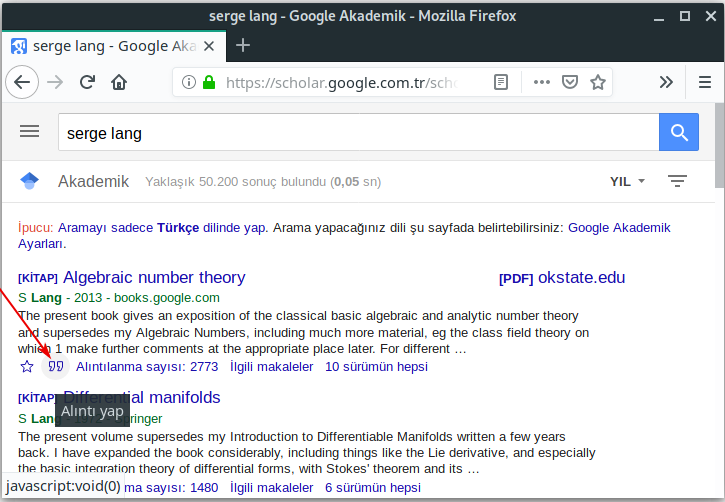
\includegraphics[width=0.33\linewidth]{images/galinti1} 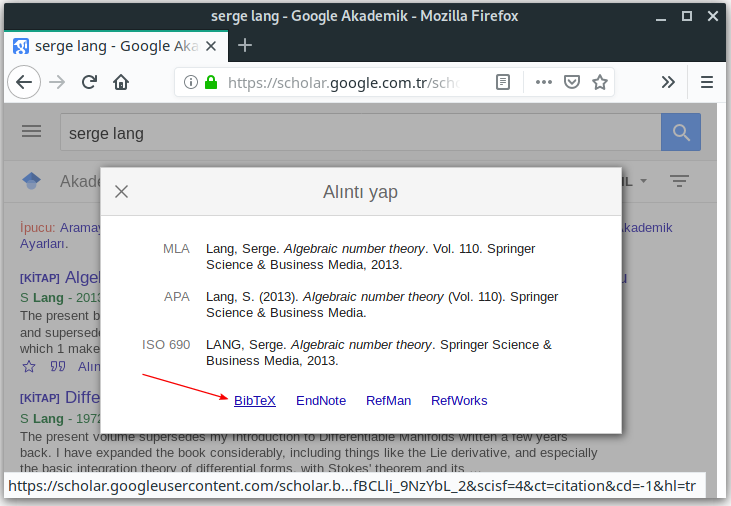
\includegraphics[width=0.33\linewidth]{images/galinti2} 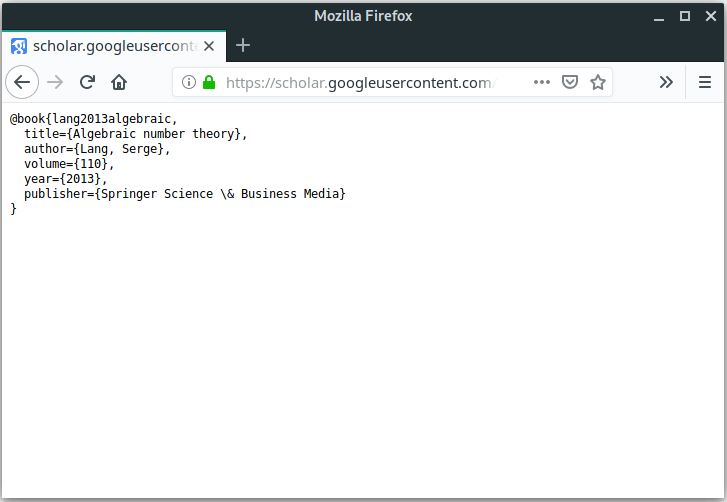
\includegraphics[width=0.33\linewidth]{images/galinti3} 

}

\caption{Google Akademikten alıntı yapma}\label{fig:fig-google}
\end{figure}

\hypertarget{dosyanux131n-hazux131rlanmasux131}{%
\subsubsection{Dosyanın hazırlanması}\label{dosyanux131n-hazux131rlanmasux131}}

Aşağıda \texttt{.bib} uzantılı bir dosya örneği gösterilmiştir.

\begin{Shaded}
\begin{Highlighting}[]
\VariableTok{@book}\NormalTok{\{}\OtherTok{lang13}\NormalTok{,}
    \DataTypeTok{title}\NormalTok{=\{Algebraic number theory\},}
    \DataTypeTok{author}\NormalTok{=\{Lang, Serge\},}
    \DataTypeTok{volume}\NormalTok{=\{110\},}
    \DataTypeTok{year}\NormalTok{=\{2013\},}
    \DataTypeTok{publisher}\NormalTok{=\{Springer Science }\CharTok{\textbackslash{}\&}\NormalTok{ Business Media\},}
\NormalTok{    \}}
\VariableTok{@article}\NormalTok{\{}\OtherTok{lamport78}\NormalTok{,}
    \DataTypeTok{title}\NormalTok{=\{Time, clocks, and the ordering of events in a}
\NormalTok{        distributed system\},}
    \DataTypeTok{author}\NormalTok{=\{Lamport, Leslie\},}
    \DataTypeTok{journal}\NormalTok{=\{Communications of the ACM\},}
    \DataTypeTok{volume}\NormalTok{=\{21\},}
    \DataTypeTok{number}\NormalTok{=\{7\},}
    \DataTypeTok{pages}\NormalTok{=\{558{-}{-}565\},}
    \DataTypeTok{year}\NormalTok{=\{1978\},}
    \DataTypeTok{publisher}\NormalTok{=\{ACM\},}
\NormalTok{\}}
\VariableTok{@manual}\NormalTok{\{}\OtherTok{Oetiker06}\NormalTok{,}
    \DataTypeTok{author}\NormalTok{ = \{Oetiker, Tobias and Partl, Hubert and Hyna, Irene}
\NormalTok{        and Schlegl, Elisabeth\},}
    \DataTypeTok{title}\NormalTok{  = \{İnce bir \{}\CharTok{\textbackslash{}LaTeXe}\NormalTok{\} Elkitabı veya, 116 dakikada}
\NormalTok{        \{}\CharTok{\textbackslash{}LaTeXe}\NormalTok{\}\},}
    \DataTypeTok{note}\NormalTok{   = \{Türkçesi: Bekir Karaoğlu\},}
    \DataTypeTok{url}\NormalTok{    = \{http://ftp.ntua.gr/mirror/ctan/info/lshort/turkish/}
\NormalTok{        lshort{-}tr.pdf\},}
    \DataTypeTok{year}\NormalTok{   = \{2006\},}
\NormalTok{\}}
\end{Highlighting}
\end{Shaded}

Bu dosyada Serge Lang'a ait bir kitap (\texttt{@book}), Leslie Lamport'a ait
bir makale (\texttt{@article}) ve LaTeX için bir teknik kılavuz (\texttt{@manual})
vardır.

Her kaynağın ilk olarak \texttt{@} işaretiyle türü belirtilir. Yukarıdakilere
ek olarak rapor için \texttt{@report}, tez için \texttt{@thesis}, çevrimiçi kaynaklar
için \texttt{@online} kullanılır. Bunların dışındaki birçok türe LaTeX
editörlerinin menü çubuğuklarında bulunan ``Kaynakça (Bibliography)''
menüsünden ulaşılabilir.

İlk girdi (\texttt{lang13}, \texttt{lamport78}, \texttt{Oetiker06}) kaynağa atıf yapmak için kullanılan anahtardır. Sonrasında
gelenler de tahmin edilebileceği gibi başlık (\texttt{title}), yazar
(\texttt{author}), yayıncı (\texttt{publisher}), yıl (\texttt{year}), dergi (\texttt{journal}), cilt
(\texttt{volume})\ldots{} gibi kaynağı tanımlayan bilgilerdir. Bu tanımlamaların her
biri eşittir işaretinden sonra iki çengelli parantez arasında yapılır
(çift tırnak da kullanılabilir) ve her tanımlama (sonuncusu olsa dahi)
virgülle ayrılır.

Yazar adı ya

\begin{Shaded}
\begin{Highlighting}[]
\CommentTok{author=\{Adı Soyadı\}}
\end{Highlighting}
\end{Shaded}

ya da

\begin{Shaded}
\begin{Highlighting}[]
\CommentTok{author=\{Soyadı, Adı\}}
\end{Highlighting}
\end{Shaded}

şeklinde girilmelidir ve birden fazla yazar varsa yazarlar yukarıdaki
yazımdan dolayı virgülle değil \texttt{and} ile ayrılmalıdır. Yazarları ayırmak
için virgül kullanırsanız yüksek ihtimalle LaTeX, yazarların adları ve
soyadlarını karıştıracaktır.

Bir diğer önemli nokta özel kelimeleri yazmak için kullanılan komutları
ve aksanlı harfleri iki çengelli
parantez içinde yazmaktır. Örneğin ``â'' için \texttt{\{\textbackslash{}\^{}a\}} yazılmalıdır. Genel
olarak sorun yaşanan karakterleri iki çengelli parantez içine yazmak
gerekir.

Her tür için zorunlu olarak belirtilmesi gereken bilgiler ve isteğe
bağlı bilgiler vardır. Bunların ne olduklarını tahmin etmek zor
değildir. Bu konuda editörden de yararlanabilirsiniz. Örneğin, \texttt{.bib}
uzantılı dosyayı açıp editörde ``Kaynakça \(\rightarrow\) Tez'' yolunu
izlerseniz aşağıdaki listeyi yazdıracaktır.

\begin{Shaded}
\begin{Highlighting}[]
\VariableTok{@thesis}\NormalTok{\{}\OtherTok{ID}\NormalTok{,}
    \DataTypeTok{author}\NormalTok{ = \{author\},}
    \DataTypeTok{title}\NormalTok{ = \{title\},}
    \DataTypeTok{type}\NormalTok{ = \{type\},}
    \DataTypeTok{institution}\NormalTok{ = \{institution\},}
    \DataTypeTok{date}\NormalTok{ = \{date\},}
    \DataTypeTok{OPTsubtitle}\NormalTok{ = \{subtitle\},}
    \DataTypeTok{OPTtitleaddon}\NormalTok{ = \{titleaddon\},}
    \DataTypeTok{OPTlanguage}\NormalTok{ = \{language\},}
    \DataTypeTok{OPTnote}\NormalTok{ = \{note\},}
    \DataTypeTok{OPTlocation}\NormalTok{ = \{location\},}
    \DataTypeTok{OPTmonth}\NormalTok{ = \{month\},}
    \DataTypeTok{OPTisbn}\NormalTok{ = \{isbn\},}
    \DataTypeTok{OPTchapter}\NormalTok{ = \{chapter\},}
    \DataTypeTok{OPTpages}\NormalTok{ = \{pages\},}
    \DataTypeTok{OPTpagetotal}\NormalTok{ = \{pagetotal\},}
    \DataTypeTok{OPTaddendum}\NormalTok{ = \{addendum\},}
    \DataTypeTok{OPTpubstate}\NormalTok{ = \{pubstate\},}
    \DataTypeTok{OPTdoi}\NormalTok{ = \{doi\},}
    \DataTypeTok{OPTeprint}\NormalTok{ = \{eprint\},}
    \DataTypeTok{OPTeprintclass}\NormalTok{ = \{eprintclass\},}
    \DataTypeTok{OPTeprinttype}\NormalTok{ = \{eprinttype\},}
    \DataTypeTok{OPTurl}\NormalTok{ = \{url\},}
    \DataTypeTok{OPTurldate}\NormalTok{ = \{urldate\},}
\NormalTok{\}}
\end{Highlighting}
\end{Shaded}

Görüldüğü gibi ilk altı satır zorunlu, OPT ile başlayanlar
isteğe bağlıdır. İsteğe bağlı olanlardan belirtmek istediklerinizin
başında bulunan OPT'yi silip tanımlamayı yapabilirsiniz.

Editörden yararlanmanın diğer bir yolu ``Kaynakça \(\rightarrow\)
Kaynakça Kaydı Ekle\ldots{}'' yolunu izlemektir. Bu yolu izlediğinizde
aşağıdaki pencere açılır (örnek TeXstudio editörüne aittir).

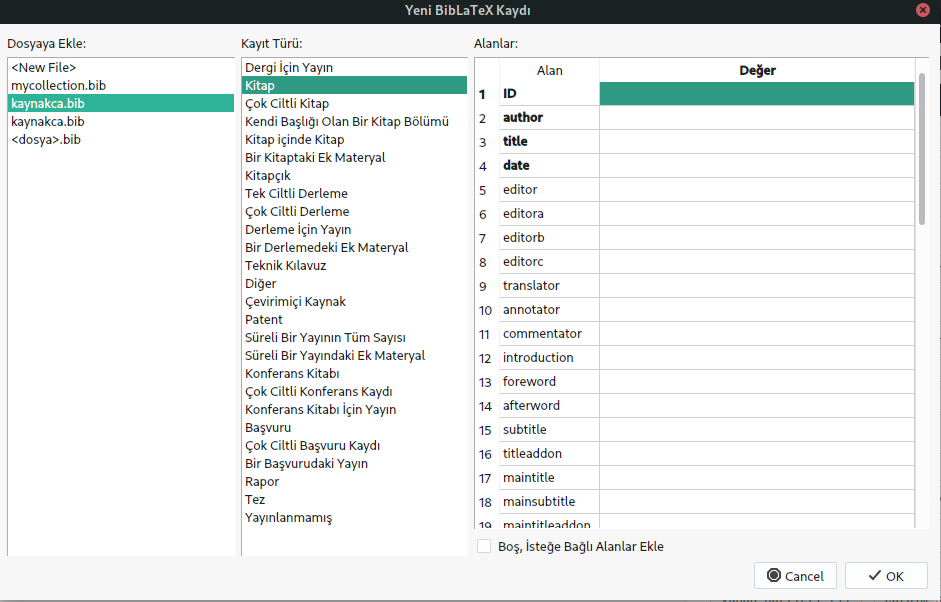
\includegraphics[width=0.6\textwidth,height=\textheight]{images/tex-studio.png}

Pencerenin solunda kaydı eklemek istediğiniz dosyayı ve ortada kayıt
türünü belirtir, sağda da kaynağın bilgilerini girersiniz. Zorunlu
bilgiler en üstte yer alan kalın yazılmış olanlardır.

\hypertarget{kaynakuxe7anux131n-yazdux131rux131lmasux131}{%
\subsubsection{Kaynakçanın yazdırılması}\label{kaynakuxe7anux131n-yazdux131rux131lmasux131}}

Kaynakçayı yazdırmak için BiBTeX'i kullanacağız. BiBTeX'in LaTeX'le
standart olarak geldiğini ifade etmiştik. Dolayısıyla bu programı
kullanmak için ek bir şey yapmanız gerekmez.

Oluşturulan \texttt{.bib} uzantılı dosya \texttt{\textbackslash{}bibliography} komutuyla içeri
aktarılır, \texttt{\textbackslash{}bibliographystyle} komutuyla da kullanılacak biçim
belirtilir.

\begin{Shaded}
\begin{Highlighting}[]
\BuiltInTok{\textbackslash{}bibliographystyle}\NormalTok{\{}\ExtensionTok{\textless{}biçim\textgreater{}}\NormalTok{\}}
\BuiltInTok{\textbackslash{}bibliography}\NormalTok{\{}\ExtensionTok{\textless{}dosya\textgreater{}}\NormalTok{\}}
\end{Highlighting}
\end{Shaded}

Burada yer alan \texttt{\textless{}dosya\textgreater{}} uzantısının belirtilmesine gerek yoktur.
Dosyanın \texttt{kaynakca.bib} olduğunu varsayarak, komut
\texttt{\textbackslash{}bibliography\{kaynakca\}} şeklinde verilir. Kullanılabilecek biçimler
\texttt{abbrv}, \texttt{acm}, \texttt{alpha}, \texttt{apalike}, \texttt{ieeetr}, \texttt{plain}, \texttt{siam} ve
\texttt{unsrt}'dir. Biçimlerin nasıl çıktı verdiklerini görmek için \href{https://tr.overleaf.com/learn/latex/Bibtex_bibliography_styles}{şuraya}
bakabilirsiniz.

Atıf, bütünleşik kaynakçada olduğu gibi \texttt{\textbackslash{}cite} komutuyla yapılır fakat
bütünleşik kaynakçadan farklı olarak atıf yapılmayan kaynaklar
yazdırılmaz. Bazı kaynakların bu kuraldan ayrı tutulması istenirse
\texttt{\textbackslash{}nocite} komutu, değişkenine kaynağın anahtarı yazılarak
\texttt{\textbackslash{}bibliography} komutundan önce verilmelidir.

\begin{Shaded}
\begin{Highlighting}[]
\KeywordTok{\textbackslash{}nocite}\NormalTok{\{}\ExtensionTok{\textless{}anahtar\textgreater{}}\NormalTok{\}}
\end{Highlighting}
\end{Shaded}

Eğer tüm kaynakların bu kuraldan ayrı tutulması isteniyorsa komut
\texttt{\textbackslash{}nocite\{*\}} şeklinde verilmelidir.

Kaynakçanın belgeye yazılması için kaynak dosyanın derlenip, BiBTeX
programının çalıştırılması ve ardından dosyanın en az iki kere daha
derlenmesi gerekir. BiBTeX programı, editörde ``Araçlar \(\rightarrow\) Kaynakça'' yoluyla çalıştırılır (klavye kısa yolu F8). Aynı şey,
uçbirimde sırasıyla

\begin{verbatim}
pdflatex kaynakdosya
bibtex kaynakdosya
pdflatex kaynakdosya
pdflatex kaynakdosya
\end{verbatim}

komutları çalıştırılarak yapılabilir.

Aşağıda kaynak dosya örneği verilmiştir. Bu dosyayı derleyebilmeniz için içeriği yukarıda verilen \texttt{kaynakca.bib} dosyasının bu dosyayla aynı dizinde olması gerektiğini unutmayınız.

\begin{Shaded}
\begin{Highlighting}[]
\BuiltInTok{\textbackslash{}documentclass}\NormalTok{[10pt,a4paper]\{}\ExtensionTok{article}\NormalTok{\}}
\BuiltInTok{\textbackslash{}usepackage}\NormalTok{[T1]\{}\ExtensionTok{fontenc}\NormalTok{\}}
\BuiltInTok{\textbackslash{}usepackage}\NormalTok{[turkish]\{}\ExtensionTok{babel}\NormalTok{\}}
\BuiltInTok{\textbackslash{}usepackage}\NormalTok{\{}\ExtensionTok{dtk{-}logos}\NormalTok{\} }\CommentTok{\% \textbackslash{}BibTeX komutu için...}
\FunctionTok{\textbackslash{}title}\NormalTok{\{Kaynakça Yönetimi 2: }\FunctionTok{\textbackslash{}BibTeX}\NormalTok{\}}
\FunctionTok{\textbackslash{}author}\NormalTok{\{Zafer Acar\}}
\KeywordTok{\textbackslash{}begin}\NormalTok{\{}\ExtensionTok{document}\NormalTok{\}}
\FunctionTok{\textbackslash{}maketitle}
\NormalTok{Lang\textquotesingle{}ın kitabı }\KeywordTok{\textbackslash{}cite}\NormalTok{\{}\ExtensionTok{lang13}\NormalTok{\}, Lamport\textquotesingle{}un makalesi  }\KeywordTok{\textbackslash{}cite}\NormalTok{\{}\ExtensionTok{lamport78}\NormalTok{\} }
\NormalTok{ve }\FunctionTok{\textbackslash{}LaTeX}\NormalTok{\{\} için Türkçe kaynak }\KeywordTok{\textbackslash{}cite}\NormalTok{\{}\ExtensionTok{Oetiker06}\NormalTok{\} }\FunctionTok{\textbackslash{}dots}

\BuiltInTok{\textbackslash{}bibliographystyle}\NormalTok{\{}\ExtensionTok{siam}\NormalTok{\}}
\BuiltInTok{\textbackslash{}bibliography}\NormalTok{\{}\ExtensionTok{kaynakca}\NormalTok{\}}
\KeywordTok{\textbackslash{}end}\NormalTok{\{}\ExtensionTok{document}\NormalTok{\}}
\end{Highlighting}
\end{Shaded}

\hypertarget{dizin}{%
\section{Dizin}\label{dizin}}

Bilimsel bir yapıtta bulunması gereken \emph{dizin} ya da diğer adıyla
\emph{indeks}, bir yapıtın kişi, konu, yer adı vb. bakımından içindekileri
yer numarasıyla belirten ve yapıtın arkasında yer alan alfabetik
listedir.

LaTeX'de dizin oluşturabilmek için sahanlığa

\begin{Shaded}
\begin{Highlighting}[]
\BuiltInTok{\textbackslash{}usepackage}\NormalTok{\{}\ExtensionTok{makeidx}\NormalTok{\}}
\FunctionTok{\textbackslash{}makeindex}
\end{Highlighting}
\end{Shaded}

komutları girilir. Birinci komut dizin için gerekli olan
\href{http://ftp.ntua.gr/mirror/ctan/macros/latex/base/makeindx.pdf}{makeidx} paketini çağırır, ikinci komut ise dizinleme
komutlarını etkinleştirir.

Dizinde gösterilmek istenen madde, \texttt{\textbackslash{}index} komutunun değişkeni olarak
girilir:

\begin{Shaded}
\begin{Highlighting}[]
\FunctionTok{\textbackslash{}index}\NormalTok{\{\textless{}madde\textgreater{}\}}
\end{Highlighting}
\end{Shaded}

Dizin maddesi girme örnekleri aşağıda gösterilmiştir.

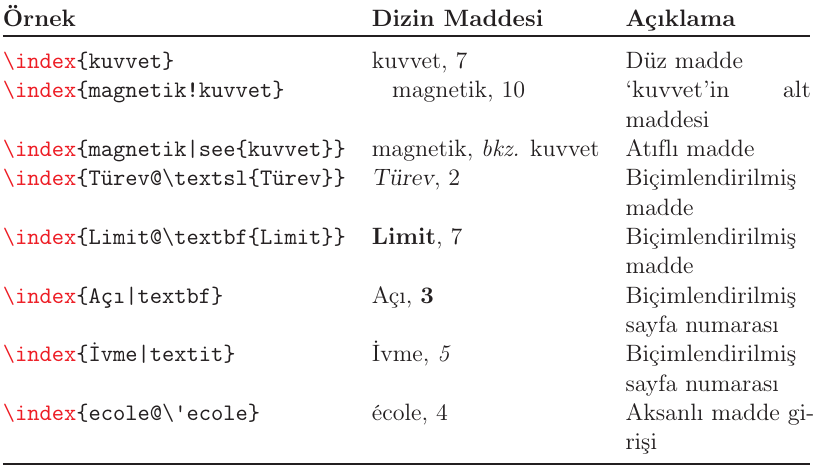
\includegraphics[width=0.9\textwidth,height=\textheight]{images/dizina.png}

LaTeX, kaynak dosyanızı derlediğinizde bu dizin maddelerini sayfa
numaralarıyla birlikte, kaynak dosyayla adı aynı fakat uzantısı \texttt{.idx}
olan bir dosyaya kaydeder (bu dosyaya \emph{ham dosya} denir). Bu dosyanın
\texttt{makeindex} programından geçirilmesi gerekir. Bu editörde ``Araçlar \(\rightarrow\) Dizin'' yoluyla yapılır. Aynı şey uçbirimde,

\begin{verbatim}
makeindex kaynakdosya
\end{verbatim}

komutu girilerek yapılabilir. Dosya tekrar derlendiğinde sıralanmış
dizin belgeye yazılır. Bunun için dizinin yazılması istenen yere
\texttt{\textbackslash{}printindex} komutu verilir. Bu genelde, belgenin en sonunda
\texttt{\textbackslash{}end\{document\}} komutundan hemen öncedir. Komutun girildiği yere LaTeX,
Türkçe dil paketi ekli belgelerde ``Dizin'' başlığını oluşturur ve belgede
\texttt{\textbackslash{}index} komutuyla eklenmiş maddeleri sırayla dizer.

Program, ham dosyayı işleyip dizin maddelerini abece sırasına göre dizer
ve \texttt{.ind} uzantılı bir dosyaya aktarır. Ancak, Türkçe aksanlı harflerle
başlayan kelimeler doğru yerde yazılmazlar. Bu harflerin doğru yere
yazılması için \texttt{.ind} uzantılı dosyanın metin editörüyle açılarak elle
düzenlenmesi gerekir. Ardından kaynak dosya derlenir. Elle düzeltmeden
sonra tekrar \texttt{makeindex} programı çalıştırılırsa \texttt{.ind} uzantılı dosya
tekrar oluşturulacağı için elle yapılan düzeltmeler bozulur. O yüzden
düzeltme en son yapılmalıdır.

\begin{quote}
Aksanlı harflerle başlayan kelimelerin doğru yerde yazılmaları için
aksanlı madde girme komutundan faydalanılabilir. Örneğin ``çekiç''
kelimesinin peşine \texttt{\textbackslash{}index\{czekiç@çekiç\}} komutu verilirse bu kelime
doğru yerde dizilecektir. Burada yapılan sorun yaratan ``ç'' harfi
yerine ``cz'' yazılmasıdır.
\end{quote}

\hypertarget{uxe7oklu-dizin}{%
\subsection{Çoklu Dizin}\label{uxe7oklu-dizin}}

Birden fazla dizin oluşturmak isterseniz (örneğin biri \emph{normal dizin}
diğeri de \emph{simgeler dizini})
\href{http://ftp.cc.uoc.gr/mirrors/CTAN/macros/latex/contrib/index/index.pdf}{index} paketini kullanabilirsiniz. Her dizin paket eklendikten ve \texttt{\textbackslash{}makeindex} komutu sahanlıkta
verildikten sonra \texttt{\textbackslash{}newindex} komutuyla tanıtılır.

\begin{Shaded}
\begin{Highlighting}[]
\BuiltInTok{\textbackslash{}usepackage}\NormalTok{\{}\ExtensionTok{index}\NormalTok{\}}
\FunctionTok{\textbackslash{}makeindex}
\FunctionTok{\textbackslash{}newindex}\NormalTok{\{normal\}\{ndx\}\{nnd\}\{Normal Dizin\}}
\FunctionTok{\textbackslash{}newindex}\NormalTok{\{simge\}\{sdx\}\{snd\}\{Simgeler Dizini\}}
\end{Highlighting}
\end{Shaded}

Komutun dört değişkeni vardır. Bunlar sırasıyla, dizin adı (örnekte
\texttt{normal} ve \texttt{simge}), oluşturulacak ham dosyanın uzantısı (örnekte
\texttt{.ndx} ve \texttt{.sdx}), \texttt{makeindex} tarafından ham dosyanın işlenmesiyle
oluşturulan dosyanın uzantısı (örnekte \texttt{.nnd} ve \texttt{.snd}) ve son olarak
\texttt{\textbackslash{}printindex} komutuyla yazdırılacak başlıktır (örnekte ``Normal Dizin''
ve ``Simgeler Dizini''). Buradaki uzantılar varsayılan \texttt{.idx} ve \texttt{.ind}
uzantılardan farklı olmalıdır.

Ardından bir kelime ya da simgeyi dizine eklemek için, eklemek istenilen
dizine göre \texttt{\textbackslash{}index} komutu köşeli parantezler içinde dizin adı
belirtilerek kullanılır.

\begin{Shaded}
\begin{Highlighting}[]
\FunctionTok{\textbackslash{}index}\NormalTok{[normal]\{kuvvet\}}
\FunctionTok{\textbackslash{}index}\NormalTok{[simge]\{F@}\SpecialStringTok{$}\SpecialCharTok{\textbackslash{}vec}\SpecialStringTok{\{F\}$}\NormalTok{\}}
\end{Highlighting}
\end{Shaded}

Birinci komut, ``kuvvet'' kelimesini normal dizine, ikinci komut \(\vec{F}\) simgesini simgeler dizinine ekler.

Belge derlendikten sonra iki tane \texttt{\textbackslash{}makeindex} komutu uçbirimde,

\begin{Shaded}
\begin{Highlighting}[]
\NormalTok{makeindex kaynakdosya.ndx {-}o kaynakdosya.nnd }
\NormalTok{makeindex kaynakdosya.sdx {-}o kaynakdosya.snd }
\end{Highlighting}
\end{Shaded}

şeklinde verilir. Belgenizde dizinlerin yazılması istenen yere de

\begin{Shaded}
\begin{Highlighting}[]
\FunctionTok{\textbackslash{}printindex}\NormalTok{[normal]}
\FunctionTok{\textbackslash{}printindex}\NormalTok{[simge]}
\end{Highlighting}
\end{Shaded}

komutları verilir. Ardından belge tekrar derlenerek dizinler yazdırılır.

Çoklu dizin için diğer bir seçenek
\href{https://www.ctan.org/pkg/multind}{multind} paketini kullanmaktır. Görece
index paketine göre daha pratiktir. Sahanlığa

\begin{Shaded}
\begin{Highlighting}[]
\BuiltInTok{\textbackslash{}usepackage}\NormalTok{\{}\ExtensionTok{multind}\NormalTok{\}}
\FunctionTok{\textbackslash{}makeindex}\NormalTok{\{normal\}}
\FunctionTok{\textbackslash{}makeindex}\NormalTok{\{simge\}}
\end{Highlighting}
\end{Shaded}

komutlarıyla \texttt{normal} ve \texttt{simge} adında iki dizin tanımlanır. Yine
dizine yazılması istenen maddeler \texttt{\textbackslash{}index} komutundan önce çengelli
parantezler içinde dizin adı belirtilerek girilir.

\begin{Shaded}
\begin{Highlighting}[]
\FunctionTok{\textbackslash{}index}\NormalTok{\{normal\}\{kuvvet\}}
\FunctionTok{\textbackslash{}index}\NormalTok{\{simge\}\{F@}\SpecialStringTok{$}\SpecialCharTok{\textbackslash{}vec}\SpecialStringTok{\{F\}$}\NormalTok{\}}
\end{Highlighting}
\end{Shaded}

Bu defa \texttt{makeindex} programı uçbirimde

\begin{Shaded}
\begin{Highlighting}[]
\NormalTok{makeindex normal}
\NormalTok{makeindex simge}
\end{Highlighting}
\end{Shaded}

komutlarıyla çalıştırılır. Yine \texttt{\textbackslash{}printindex} komutları dizinlerin
eklenmesi istenen yere

\begin{Shaded}
\begin{Highlighting}[]
\FunctionTok{\textbackslash{}printindex}\NormalTok{\{normal\}\{Normal Dizin\}}
\FunctionTok{\textbackslash{}printindex}\NormalTok{\{simge\}\{Simgeler Dizini\}}
\end{Highlighting}
\end{Shaded}

şeklinde verilir.

\hypertarget{dizinin-iuxe7indekiler-tablosuna-yazux131lmasux131}{%
\subsection{Dizinin İçindekiler tablosuna yazılması}\label{dizinin-iuxe7indekiler-tablosuna-yazux131lmasux131}}

Dizini İçindekiler tablosuna yazmak için \texttt{\textbackslash{}printindex} komutunun peşine
\texttt{book} ve \texttt{report} sınıflarında \texttt{\textbackslash{}addcontentsline} komutu,

\begin{Shaded}
\begin{Highlighting}[]
\FunctionTok{\textbackslash{}addcontentsline}\NormalTok{\{toc\}\{chapter\}\{}\FunctionTok{\textbackslash{}indexname}\NormalTok{\}}
\end{Highlighting}
\end{Shaded}

şeklinde, \texttt{article} sınıfında ise

\begin{Shaded}
\begin{Highlighting}[]
\FunctionTok{\textbackslash{}addcontentsline}\NormalTok{\{toc\}\{section\}\{}\FunctionTok{\textbackslash{}indexname}\NormalTok{\}}
\end{Highlighting}
\end{Shaded}

şeklinde verilmelidir. Çoklu dizin oluşturulmuşsa, \texttt{book} ve \texttt{report}
sınıflarında

\begin{Shaded}
\begin{Highlighting}[]
\FunctionTok{\textbackslash{}printindex}\NormalTok{\{normal\}\{Normal Dizin\}}
\FunctionTok{\textbackslash{}addcontentsline}\NormalTok{\{toc\}\{chapter\}\{Normal Dizin\}}
\FunctionTok{\textbackslash{}printindex}\NormalTok{\{simge\}\{Simgeler Dizini\}}
\FunctionTok{\textbackslash{}addcontentsline}\NormalTok{\{toc\}\{chapter\}\{Simgeler Dizini\}}
\end{Highlighting}
\end{Shaded}

şeklinde, \texttt{article} sınıfında ise komutlardaki \texttt{chapter} yazan yere
\texttt{section} yazarak verilmelidir.

\backmatter

  \bibliography{book.bib,packages.bib}

\printindex

\end{document}
